\documentclass[a4paper,12pt,twoside]{memoir}
\usepackage[left=4cm,right=3cm]{geometry}
\usepackage{xr}
% Castellano
\usepackage[spanish,es-tabla]{babel}
\selectlanguage{spanish}
\usepackage[utf8]{inputenc}
\usepackage[T1]{fontenc}
\usepackage{lmodern} % Scalable font
\usepackage{microtype}
\usepackage{placeins}

\RequirePackage{booktabs}
\RequirePackage[table]{xcolor}
\RequirePackage{xtab}
\RequirePackage{multirow}

% Links
\PassOptionsToPackage{hyphens}{url}\usepackage[colorlinks]{hyperref}
\hypersetup{
	allcolors = {red}
}

% Ecuaciones
\usepackage{amsmath}

% Rutas de fichero / paquete
\newcommand{\ruta}[1]{{\sffamily #1}}

% Párrafos
\nonzeroparskip

% Huérfanas y viudas
\widowpenalty100000
\clubpenalty100000

% Imagenes
\usepackage{graphicx}
\newcommand{\imagen}[2]{
	\begin{figure}[!h]
		\centering
		\includegraphics[width=0.9\textwidth]{#1}
		\caption{#2}\label{fig:#1}
	\end{figure}
	\FloatBarrier
}

\newcommand{\imagenflotante}[2]{
	\begin{figure}%[!h]
		\centering
		\includegraphics[width=0.9\textwidth]{#1}
		\caption{#2}\label{fig:#1}
	\end{figure}
}



% El comando \figura nos permite insertar figuras comodamente, y utilizando
% siempre el mismo formato. Los parametros son:
% 1 -> Porcentaje del ancho de página que ocupará la figura (de 0 a 1)
% 2 --> Fichero de la imagen
% 3 --> Texto a pie de imagen
% 4 --> Etiqueta (label) para referencias
% 5 --> Opciones que queramos pasarle al \includegraphics
% 6 --> Opciones de posicionamiento a pasarle a \begin{figure}
\newcommand{\figuraConPosicion}[6]{%
  \setlength{\anchoFloat}{#1\textwidth}%
  \addtolength{\anchoFloat}{-4\fboxsep}%
  \setlength{\anchoFigura}{\anchoFloat}%
  \begin{figure}[#6]
    \begin{center}%
      \Ovalbox{%
        \begin{minipage}{\anchoFloat}%
          \begin{center}%
            \includegraphics[width=\anchoFigura,#5]{#2}%
            \caption{#3}%
            \label{#4}%
          \end{center}%
        \end{minipage}
      }%
    \end{center}%
  \end{figure}%
}

%
% Comando para incluir imágenes en formato apaisado (sin marco).
\newcommand{\figuraApaisadaSinMarco}[5]{%
  \begin{figure}%
    \begin{center}%
    \includegraphics[angle=90,height=#1\textheight,#5]{#2}%
    \caption{#3}%
    \label{#4}%
    \end{center}%
  \end{figure}%
}
% Para las tablas
\newcommand{\otoprule}{\midrule [\heavyrulewidth]}
%
% Nuevo comando para tablas pequeñas (menos de una página).
\newcommand{\tablaSmall}[5]{%
 \begin{table}
  \begin{center}
   \rowcolors {2}{gray!35}{}
   \begin{tabular}{#2}
    \toprule
    #4
    \otoprule
    #5
    \bottomrule
   \end{tabular}
   \caption{#1}
   \label{tabla:#3}
  \end{center}
 \end{table}
}

%
% Nuevo comando para tablas pequeñas (menos de una página).
\newcommand{\tablaSmallSinColores}[5]{%
 \begin{table}[H]
  \begin{center}
   \begin{tabular}{#2}
    \toprule
    #4
    \otoprule
    #5
    \bottomrule
   \end{tabular}
   \caption{#1}
   \label{tabla:#3}
  \end{center}
 \end{table}
}

\newcommand{\tablaApaisadaSmall}[5]{%
\begin{landscape}
  \begin{table}
   \begin{center}
    \rowcolors {2}{gray!35}{}
    \begin{tabular}{#2}
     \toprule
     #4
     \otoprule
     #5
     \bottomrule
    \end{tabular}
    \caption{#1}
    \label{tabla:#3}
   \end{center}
  \end{table}
\end{landscape}
}

%
% Nuevo comando para tablas grandes con cabecera y filas alternas coloreadas en gris.
\newcommand{\tabla}[6]{%
  \begin{center}
    \tablefirsthead{
      \toprule
      #5
      \otoprule
    }
    \tablehead{
      \multicolumn{#3}{l}{\small\sl continúa desde la página anterior}\\
      \toprule
      #5
      \otoprule
    }
    \tabletail{
      \hline
      \multicolumn{#3}{r}{\small\sl continúa en la página siguiente}\\
    }
    \tablelasttail{
      \hline
    }
    \bottomcaption{#1}
    \rowcolors {2}{gray!35}{}
    \begin{xtabular}{#2}
      #6
      \bottomrule
    \end{xtabular}
    \label{tabla:#4}
  \end{center}
}

%
% Nuevo comando para tablas grandes con cabecera.
\newcommand{\tablaSinColores}[6]{%
  \begin{center}
    \tablefirsthead{
      \toprule
      #5
      \otoprule
    }
    \tablehead{
      \multicolumn{#3}{l}{\small\sl continúa desde la página anterior}\\
      \toprule
      #5
      \otoprule
    }
    \tabletail{
      \hline
      \multicolumn{#3}{r}{\small\sl continúa en la página siguiente}\\
    }
    \tablelasttail{
      \hline
    }
    \bottomcaption{#1}
    \begin{xtabular}{#2}
      #6
      \bottomrule
    \end{xtabular}
    \label{tabla:#4}
  \end{center}
}

%
% Nuevo comando para tablas grandes sin cabecera.
\newcommand{\tablaSinCabecera}[5]{%
  \begin{center}
    \tablefirsthead{
      \toprule
    }
    \tablehead{
      \multicolumn{#3}{l}{\small\sl continúa desde la página anterior}\\
      \hline
    }
    \tabletail{
      \hline
      \multicolumn{#3}{r}{\small\sl continúa en la página siguiente}\\
    }
    \tablelasttail{
      \hline
    }
    \bottomcaption{#1}
  \begin{xtabular}{#2}
    #5
   \bottomrule
  \end{xtabular}
  \label{tabla:#4}
  \end{center}
}



\definecolor{cgoLight}{HTML}{EEEEEE}
\definecolor{cgoExtralight}{HTML}{FFFFFF}

%
% Nuevo comando para tablas grandes sin cabecera.
\newcommand{\tablaSinCabeceraConBandas}[5]{%
  \begin{center}
    \tablefirsthead{
      \toprule
    }
    \tablehead{
      \multicolumn{#3}{l}{\small\sl continúa desde la página anterior}\\
      \hline
    }
    \tabletail{
      \hline
      \multicolumn{#3}{r}{\small\sl continúa en la página siguiente}\\
    }
    \tablelasttail{
      \hline
    }
    \bottomcaption{#1}
    \rowcolors[]{1}{cgoExtralight}{cgoLight}

  \begin{xtabular}{#2}
    #5
   \bottomrule
  \end{xtabular}
  \label{tabla:#4}
  \end{center}
}



\graphicspath{ {./img/} }

% Capítulos
\chapterstyle{bianchi}
\newcommand{\capitulo}[2]{
	\setcounter{chapter}{#1}
	\setcounter{section}{0}
	\setcounter{figure}{0}
	\setcounter{table}{0}
	\chapter*{#2}
	\addcontentsline{toc}{chapter}{#2}
	\markboth{#2}{#2}
}

% Apéndices
\renewcommand{\appendixname}{Apéndice}
\renewcommand*\cftappendixname{\appendixname}

\newcommand{\apendice}[1]{
	%\renewcommand{\thechapter}{A}
	\chapter{#1}
}

\renewcommand*\cftappendixname{\appendixname\ }

% Formato de portada
\makeatletter
\usepackage{xcolor}
\newcommand{\tutor}[1]{\def\@tutor{#1}}
\newcommand{\course}[1]{\def\@course{#1}}
\definecolor{cpardoBox}{HTML}{E6E6FF}
\def\maketitle{
  \null
  \thispagestyle{empty}
  % Cabecera ----------------
\noindent
\includegraphics[width=\textwidth]{cabecera}\vspace{1cm}%
  \vfill
  % Título proyecto y escudo informática ----------------
  \colorbox{cpardoBox}{%
    \begin{minipage}{.8\textwidth}
      \vspace{.5cm}\Large
      \begin{center}
      \textbf{TFG del Grado en Ingeniería Informática}\vspace{.6cm}\\
      \textbf{\LARGE\@title{}}
      \end{center}
      \vspace{.2cm}
    \end{minipage}

  }%
  \hfill\begin{minipage}{.20\textwidth}
    
\includegraphics[width=\textwidth]{escudoInfor}
  \end{minipage}
    \vspace{0.2cm}
	\begin{figure}[h!]
		\centering
		
\includegraphics[scale=0.4]{img/Logo_TheOnlyOne.png}
	\end{figure}
  % Datos de alumno, curso y tutores ------------------
  \begin{center}%
  {%
    \noindent\LARGE
    Presentado por \@author{}\\ 
    en Universidad de Burgos --- \@date{}\\
    Tutor: \@tutor{}\\
  }%
  \end{center}%
  \null
  \cleardoublepage
  }
\makeatother

\newcommand{\nombre}{Alberto Fuente Robles} %%% cambio de comando

% Datos de portada
\title{``The Only One'': Desarrollo de un videojuego 3D Battle Royale en Unity}
\author{\nombre}
\tutor{Jesús Manuel Maudes Raedo}
\date{\today}

\begin{document}

\maketitle


\newpage\null\thispagestyle{empty}\newpage


%%%%%%%%%%%%%%%%%%%%%%%%%%%%%%%%%%%%%%%%%%%%%%%%%%%%%%%%%%%%%%%%%%%%%%%%%%%%%%%%%%%%%%%%
\thispagestyle{empty}


\noindent
\includegraphics[width=\textwidth]{cabecera}\vspace{1cm}

\noindent D. Jesús Manuel Maudes Raedo, profesor del departamento de Ingeniería Informática, área de Lenguajes y Sistemas Informáticos.

\noindent Expone:

\noindent Que el alumno D. \nombre, con DNI 71302832A, ha realizado el Trabajo final de Grado en Ingeniería Informática titulado ``The Only One'': Desarrollo de un videojuego 3D Battle Royale en Unity. 

\noindent Y que dicho trabajo ha sido realizado por el alumno bajo la dirección del que suscribe, en virtud de lo cual se autoriza su presentación y defensa.

\begin{center} %\large
En Burgos, {\large \today}
\end{center}

\vfill\vfill\vfill

% Author and supervisor
\begin{minipage}{0.45\textwidth}
\begin{flushleft} %\large
Vº. Bº. del Tutor:\\[2cm]
D. nombre tutor
\end{flushleft}
\end{minipage}
\hfill
\begin{minipage}{0.45\textwidth}
\begin{flushleft} %\large
Vº. Bº. del co-tutor:\\[2cm]
D. nombre co-tutor
\end{flushleft}
\end{minipage}
\hfill

\vfill

% para casos con solo un tutor comentar lo anterior
% y descomentar lo siguiente
%Vº. Bº. del Tutor:\\[2cm]
%D. nombre tutor


\newpage\null\thispagestyle{empty}\newpage




\frontmatter

% Abstract en castellano
\renewcommand*\abstractname{Resumen}
\begin{abstract}
``The Only One'' es un proyecto con el que se pretende abarcar el desarrollo completo de un videjouego 3D de la mano de Unity junto con otras herramientas de creación.

En este shooter en primera persona, se controlará a un humano que debe luchar por mantenerse con vida en un mundo desconocido repleto de robots que quieren acabar con él.

A través de este trabajo se abordará todo el proceso de su desarrollo, desde las fases iniciales, hasta la obtención de una versión completa y jugable del videojuego.
\end{abstract}

\renewcommand*\abstractname{Descriptores}
\begin{abstract}
Videojuego, shooter, battle royale, Unity, C\#
\end{abstract}

\clearpage

% Abstract en inglés
\renewcommand*\abstractname{Abstract}
\begin{abstract}
``The Only One'' is a project that aims to reach the complete development of a 3D video game with the help of Unity and other creation tools.

In this first person shooter, you will control a human who must fight to stay alive in an unknown world full of robots that want to kill you.

Through this work the whole process of its development will be explained, from the initial stages until obtaining a complete and playable version of the game.
\end{abstract}

\renewcommand*\abstractname{Keywords}
\begin{abstract}
Video game, shooter, battle royale, Unity, C\#
\end{abstract}

\clearpage

% Indices
\tableofcontents

\clearpage

\listoffigures

\clearpage

\listoftables
\clearpage

\mainmatter
\capitulo{1}{Introducción}

Los videojuegos son productos software enfocados al entretenimiento que simulan experiencias a través de una pantalla, y que, a diferencia de otras formas de ocio, requieren de la interacción activa del usuario a través de alguna forma de control, como un \textit{joystick}, un teclado y un ratón, o sus propias manos, para que sucedan eventos y acciones dentro del videojuego a gusto del jugador. De esta forma, el usuario se convierte en parte activa de la realidad virtual en la que está inmerso y puede sentir que tiene el control de lo que sucede mientras vive experiencias muy variadas.

Y es precisamente esa variedad que tienen los videojuegos en cuanto a su complejidad, calidad gráfica, temática, estilo artístico, género, historia narrativa, e incluso rango de precio, lo que ha hecho que en los últimos años se hayan convertido en un producto masivo, con el que un público cada vez más amplio puede disfrutar de todo tipo de experiencias jugables acorde a sus gustos y preferencias.

A esto se le suma el gran avance tecnológico que han sufrido recientemente los distintas dispositivos electrónicos, convirtiéndose en máquinas cada vez más potentes, lo que da como resultado que cualquiera pueda disfrutar de una partida a su juego favorito donde, cuando y como desee, ya sea en ordenadores, móviles, tabletas, o claro está, en las amadas consolas.

Los videojuegos tienen más alcance y popularidad que nunca. Se han convertido en una de las formas de entretenimiento más importantes y extendidas en todo el mundo, lo que también ha provocado que sea actualmente una de las industrias que más dinero genera.
Según estima el último informe de \textit{Accenture} \cite{wiki:videojuegos}, el valor total de la industria de los videojuegos está por encima de los 245.000 millones de euros y ha superado ya a las industrias del cine y la música juntas.

Teniendo en cuenta estos datos, no es de extrañar que la popularidad de los videojuegos no se haya visto incrementada sólo en el lado de los jugadores, sino también en el de los desarrolladores de software, que han visto una oportunidad para crear productos únicos que atraigan a todo tipo de personas.

No obstante, los videojuegos son productos muy particulares que involucran diferentes ámbitos, como la programación, el modelado, el diseño de interfaces, el arte, la música, el diseño de espacios, la animación o la capacidad narrativa, entre otros.                                                   
Es este sentimiento de desafío, unido a la curiosidad y a la pasión por los videojuegos la que ha llevado al alumno a querer entender el proceso de desarrollar  un videojuego desde la perspectiva del programador de software y los retos que ello conlleva.


\section{Materiales adjuntos}

El proyecto está formado por los siguientes materiales:
\begin{itemize}
\item Conjunto de archivos que forman la aplicación \textbf{``The Only One''} para Windows y Linux.
\item Repositorio de Github con los códigos fuente y resto archivos necesarios para su edición en el motor de Unity.
\item Vídeo explicativo del uso del videojuego.
\item Memoria del Trabajo de Fin de Grado
\item Anexos del proyecto
\end{itemize}

\section{Estructura de la memoria}

La memoria consta de los siguientes puntos a tratar:
\begin{itemize}
\item \textbf{Introducción.} Breve contexto y descripción del proyecto, así como los materiales y la estructura de la memoria.
\item \textbf{Objetivos del proyecto.} Enumeración de los objetivos principales que se persiguen con el proyecto.
\item \textbf{Conceptos teóricos.} Explicación de los términos y conceptos en relación a la materia que se trata, esenciales para comprender el desarrollo del proyecto.
\item \textbf{Técnicas y herramientas.} Descripción de las técnicas, herramientas y programas utilizados durante el desarrollo del proyecto.
\item \textbf{Aspectos relevantes.} Explicación de los aspectos más interesantes que tuvieron lugar durante el desarrollo del proyecto, así como las cuestiones y dificultades más destacables que surgieron y cómo se abordaron.
\item \textbf{Trabajos relacionados.} Breve descripción de trabajos y productos de similar naturaleza al proyecto que se expone.
\item \textbf{Conclusiones y Líneas de trabajo futuras.} Exposición de las conclusiones obtenidas una vez finalizado el desarrollo del proyecto, así como los pasos a seguir en el futuro para la mejora del producto desarrollado.
\end{itemize}
\capitulo{2}{Objetivos del proyecto}

A continuación se describen los objetivos que se pretenden alcanzar con el desarrollo de este proyecto:
\begin{itemize}
\tightlist
	\item Desarrollar un videojuego de género \textit{shooter}, en concreto del estilo \textit{battle royale}, para ordenador como plataforma de juego, compatible con Windows y Linux y pensado para controlarse con teclado y ratón. Este objetivo puede subdividirse a su vez en objetivos más concretos:
    	\begin{itemize}
    	\tightlist
    	\item Desarrollar una buena \textbf{jugabilidad} y mecánicas interesantes para que el producto resulte entretenido y divertido para los usuarios.
    	\item Hacer que el producto sea \textbf{accesible} para un gran espectro de usuarios, es decir, que aprendan las mecánicas y acciones que ofrece el videojuego de forma intuitiva y con una curva de aprendizaje sencilla y no frustrante.
    	\item Crear de manera \textbf{autónom}a la mayoría de componentes del videojuego, incluyendo scripts, modelos, texturas, efectos, elementos de interfaces y sonidos.
    	\item Hacer que el videojuego sea \textbf{óptimo} en términos de rendimiento.
    	\item Utilizar \textbf{patrones, algoritmos y estructuras} de programación convenientes en cada caso.
    	\item Hacer que el proyecto sea fácilmente \textbf{extensible} para incluir mecánicas, objetos, mejoras o modificaciones de manera sencilla e intuitiva.
    	\end{itemize}
	\item Aprender el funcionamiento y las características fundamentales de Unity, así como del lenguaje de programación que utiliza (C\#)
	\item Aplicar la metodología \textit{Kanban} durante el desarrollo del producto para la gestión de las tareas.
	\item Integrar Git y Github como sistema de control de versiones.
	\item Asentar las bases de conocimiento personal para poder realizar otros proyectos similares en el futuro o continuar el desarrollo y mejora del mismo.
\end{itemize}
\capitulo{3}{Conceptos teóricos} \label{Conceptos teóricos}
En esta sección se definen algunos términos y conceptos importantes en relación a la materia que se trata, que pueden resultar de gran ayuda a la hora de comprender los diferentes aspectos que conforman el desarrollo del proyecto.
\section{Motor de videojuegos}
Un motor de videojuegos o \textit{game engine} es un framework o conjunto de librerías y utilidades de programación que permite agilizar el proceso de creación y desarrollo de un videojuego, desde su diseño, programación y construcción, hasta su compilación y ejecución \cite{wiki:motor_de_videojuegos}.

El motor provee herramientas al programador para que pueda enfocarse en el desarrollo del videojuego en sí, en lugar de dedicar tanto tiempo a aspectos más generales y de bajo nivel, tales como el sistema de físicas, el sistema de sonido o la representación de las imágenes en la pantalla.

Existen diversos motores de videojuegos disponibles en el mercado, pero entre los más populares destacan \textit{Unreal Engine}, \textit{Unity}, \textit{Frostbite Engine}, \textit{Cry Engine} y \textit{Decima Engine}.
Algunas de las herramientas principales que proporciona un motor de videojuegos son las que se describen a continuación:
\subsection{Motor gráfico}
El motor gráfico es el componente del motor de videojuegos más importante y, de hecho, suelen confundirse ambos términos entre ellos. Se encarga del renderizado de las imágenes, dibujando todos los aspectos gráficos en la pantalla, es decir, mostrando las imágenes que componen cada instante en la escena mediante el cálculo de los polígonos, la iluminación o las texturas, y la interacción que hay entre ellos. 

Normalmente el renderizado se basa en alguna API gráfica, como \textit{OpenGL}, \textit{Directx} o \textit{Vulkan}, ya que proporcionan abstracciones software de la GPU (\textit{Graphics Processing Unit}) y también accesos a componentes hardware independientemente de la plataforma que se utilice.
\subsection{Motor de físicas}
El motor de físicas es la parte del motor de videojuegos que hace posible aplicar aproximaciones físicas a los diferentes objetos del videojuego para generar una sensación más realista cuando interactúen entre ellos o con el entorno. Es decir, es el encargado de realizar los cálculos necesarios para que un objeto simule tener atributos físicos como masa, volumen, fricción, aceleración, gravedad, y se puedan aplicar fuerzas y colisiones sobre ellos.
\subsection{Motor de sonidos}
El motor de sonidos se encarga de cargar, adaptar y gestionar todas las pistas de audio que necesite el videojuego, como efectos de sonido, diálogos o música. Gracias a él se pueden reproducir, detener, sincronizar los sonidos, así como aplicar diversos efectos sobre ellas, como la reverberación o un filtrado de sus propiedades como el volumen, el tono o su comportamiento espacial.

\section{Conceptos propios de Unity}
El motor elegido para el proyecto ha sido \textbf{Unity} (más adelante se explicarán los motivos), por lo que se procederá a explicar algunos conceptos y términos sobre esta herramienta esenciales para entender su funcionamiento:
\subsection{Asset}
Un Asset \cite{doc:Asset} es una representación que Unity hace de cualquier tipo de archivo que pueda ser utilizado en el proyecto. Pueden ser propios de Unity como scripts o materiales, o bien importarse de forma externa al motor, como modelos 3D, archivos de audio, imágenes, etc. Los assets son los componentes o ingredientes que se combinarán con herramientas del propio motor para crear los diferentes elementos que conformarán el videojuego.
\subsection{Scene}
Una escena o \textit{Scene} \cite{doc:Scene} es el  espacio tridimensional virtual que contiene los distintos elementos del juego. Puede haber varias escenas en un mismo proyecto para poder crear los diferentes niveles o pantallas que componen el juego. Por ejemplo, se puede tener una escena dedicada al menú principal y otra a un nivel jugable, cada una con diferentes elementos según el objetivo de dicha escena.

Las escenas se almacenan como un asset más del videojuego. Al cargar una nueva escena en tiempo de ejecución, la escena antigua se destruirá, al igual que todos los objetos contenidos en ella, a excepción de que se llame al método \textit{DontDestroyOnLoad()} \cite{doc:DontDestroyOnLoad}, pasándole como parámetro el objeto que queremos que no se destruya cuando se carga una nueva escena.
\subsection{GameObject}
Un \textit{gameobject} \cite{doc:GameObject} es un término que se usa para referirse a cada entidad u objeto del juego. Estos constituyen la base para crear cualquier tipo de elemento dentro de una escena. Funcionan como contenedores a los que se les pueden añadir diferentes componentes que definen y controlan su comportamiento. Por ejemplo, el gameobject del jugador contendrá componentes y propiedades diferentes al gameobject de un árbol, ya que tienen funciones y comportamientos distintos.

Los Gameobjects, por defecto, tiene asignados algunos atributos, entre los que destacan \textbf{\textit{name}} usado para identificar el gameobject fácilmente, \textbf{\textit{tag}} si se desea marcar con alguna etiqueta predefinida para clasificarlo de manera especial, o \textbf{\textit{layer}}, para incluir cada gameobject en una capa determinada. Este último es útil si queremos realizar acciones sólo en unas capas determinadas e ignorar otras. Por ejemplo, cuando se dispara con algún arma, se ignora la capa “weapon”, a la que pertenece el propio arma, para evitar que el “proyectil” colisione con el propio arma.

La clase GameObject tiene varios métodos, entre los que se pueden destacar \textbf{\textit{GetComponent()}} \cite{doc:GetComponent}, que permite al gameobject acceder a través de un script a todos sus componentes para poder controlarlos, y \textbf{\textit{SetActive()}} \cite{doc:SetActive}, que activa o desactiva el GameObject según el parámetro booleano que se le pase por parámetro. Desactivar un GameObject desactiva automáticamente todos sus componentes hasta que se vuelva a activar.

Además de estos métodos, existen otros propios de la clase Monobehaviour \ref{Monobehaviour} que también están muy ligados a los gameobjects, y son:
\begin{itemize}
\tightlist
	\item \textbf{\textit{OnEnable()}} \cite{doc:OnEnable}: Se ejecuta cuando un se activa un gameobject.
	\item \textbf{\textit{OnDisable()}} \cite{doc:OnDisable}: Es el último método en ejecutarse antes de que se desactive el gameobject.
\end{itemize}

También se deben mencionar dos métodos importantes de la clase \textit{Object}, que es la clase raíz de todas las clases de la jerarquía. Estos métodos son:
\begin{itemize}
\tightlist
	\item \textbf{\textit{Instantiate()}} \cite{doc:Instantiate} Permite crear ``clones'' de un gameobject concreto. Este método es muy conveniente en conjunción con los prefabs (explicados más adelante) para crear nuevas instancias de un objeto personalizado.
	\item \textbf{\textit{Destroy()}} \cite{doc:Destroy} Destruye un componente o gameobject concreto. Se puede destruir instantáneamente o tras un retardo especificado por parámetro. Al llamarlo en un gameobject, también se destruyen sus componentes y sus hijos en caso de quelos tuviera, y se ejecuta el método \textbf{\textit{OnDestroy()}} \cite{doc:OnDestroy} justo antes de que se elimine definitivamente. En ella se suelen hacer tareas de limpieza relacionadas con el gameobject.
\end{itemize}	
El método Destroy() es recurrente en el proyecto por ejemplo al instanciar partículas u otros elementos, destruyéndolos tras unos segundos para que no se mantengan en la escena durante mucho tiempo y así no sobrecargar la memoria de la aplicación.
\subsection{Components}
Los componentes de Unity \cite{doc:Components} son piezas modulares que pueden adherirse a un gameobject para dotarlo de distintas funciones, capacidades y comportamientos según se requiera. A su vez, cada componente posee diferentes referencias y propiedades que se pueden ajustar en el editor o a través de scripts para adecuar el comportamiento del gameobject a las necesidades del proyecto.

Cada gameobject puede tener varios componentes, y existen una amplia variedad de ellos, como físicos, de renderizado, sonoros o propios de las interfaces. No obstante, cuando se quieren definir comportamientos más complejos en los objetos, o bien relaciones entre ellos, se pueden crear mediante \textit{scripting}, explicado en el apartado \ref{Scripting}, y que también se pueden ligar a un gameobject como un componente más.
\begin{figure}[h]
	\centering
	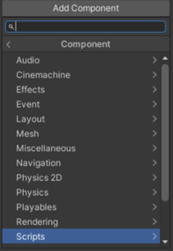
\includegraphics[scale=1]{img/addComponent.png}
	\caption{Añadir un componente a un gameobject}
	\label{fig:componente}
\end{figure}
Algunos de los más componentes predefinidos en Unity más utilizados en el proyecto son los siguientes:
\begin{itemize}
\tightlist
\item \textbf{\textit{Transform}} \cite{doc:Transform}: Este componente lo tienen por defecto todos los gameobjects del juego, y define su tamaño, rotación y posición. Algo a destacar es que los valores de este componente son relativos al contenedor inmediatamente superior del gameObject. Es decir, no es comparable el componente Transform de un gameObject independiente, cuyo contenedor inmediato es la propia escena o el ``mundo'', que el Transform de un gameobject contenido en otro. En este caso su Transform será relativo al gameobject padre.
\item \textbf{\textit{MeshRenderer}}\cite{doc:Transform}:Se encarga de renderizar la malla definida por otro componente llamado \textit{Mesh Filter}, que se encarga de construir una malla desde los assets. Por lo tanto, su función consiste en mostrar las mallas de polígonos en pantalla, teniendo en cuenta el \textit{Transform} del objeto, la luz y otros factores.
\item \textbf{\textit{Collider}}\cite{doc:Collider}: Define el área de colisión de un objeto ante interacciones físicas. Es invisible, y normalmente se utiliza un collider con una forma genérica, como un cubo o una esfera, para aproximarse al volumen del objeto, sin que tenga que ser exacto, para así mejorar el rendimiento general del juego.
Un collider especial es el \textbf{\textit{MeshCollider}}, el cual sí se intenta adaptar lo máximo posible a la geometría original del objeto al que está ligado. Por ejemplo, si el suelo no es plano sino que tiene irregularidades, valles y resaltos, como es el caso, es importante que el collider se adapte bien a su forma para que en todo momento el jugador se pueda apoyar fielmente sobre su superficie.

Además, los colliders pueden tener su propiedad \textit{IsTrigger} marcada, lo que hará que deje de registrar colisiones físicas, y en su lugar se convierta en un ``disparador'' que mandará una señal cuando otro objeto entre o salga de su área de actuación para así poder controlar las acciones que se le indiquen a través de scripts.
\item \textbf{\textit{Rigidbody}}\cite{doc:Rigidbody}: Este componente hace que el movimiento del gameobject sea controlado por físicas, es decir, que pueda ser afectado por la gravedad y otras fuerzas. En conjunción con un collider, el gameobject se verá afectado por las colisiones con otros objetos de manera fiel a como ocurriría en el mundo real.

El jugador, por ejemplo, tiene tanto un rigidbody como un collider, y su movimiento es controlado por fuerzas físicas en lugar de ser desplazado modificando su componente Transform. Esto otorga un mayor realismo de movimiento y de interacción con el entorno

\item \textbf{\textit{AudioSource}}\cite{doc:AudioSource}: Indica que el gameobject puede producir sonidos. Los sonidos emitidos por los gameobjects con este componente pueden ser recogidos por por el componente \textbf{\textit{AudioListener}}. Este debe ser único en la escena y normalmente se encuentra en la cámara principal del juego, al menos en los juegos en primera persona, ya que la cámara actúa como los ojos del jugador, y gracias a este componente, también representaría sus oídos.
\item \textbf{\textit{Animator}}\cite{doc:Animator}: El componente Animator se utiliza para asignar una o varias animaciones a un gameobject. Requiere una referencia a un \textbf{\textit{Animator Controller}}, un  tipo de asset que gestiona el conjunto de clips de animación que puede utilizar, dictando cuándo se debe reproducir cada uno, cómo se mezclan y cómo se transiciona de uno a otro.	
\end{itemize}
\subsection{Prefab}
Un prefab \cite{doc:Prefabs} es un tipo de asset que almacena un gameobject completo, incluyendo sus componentes y propiedades. Actúa como una plantilla reutilizable a partir de la cual se pueden crear nuevas instancias de ese objeto en la escena. De esta manera, si se desea tener varios objetos idénticos, no se tienen que construir todos de cero.\\ Además, si se modifica el prefab, se modificarán automáticamente todas las instancias que existan de él en la escena, lo que resulta muy conveniente a la hora de mejorar o editar varios elementos de forma sencilla y eficiente.
Por ejemplo, este proyecto dispone de un prefab por cada objeto del que se espera más de una copia, como los enemigos, las cajas de suministros, las armas, o los objetos decorativos, entre otros.
\subsection{Shader}
Un shader \cite{doc:Shader} es un conjunto de instrucciones que ejecuta la GPU para definir cómo se deben de renderizar o mostrar los materiales asociados a los objetos.
A partir de un shader se pueden crear varios materiales configurando sus parámetros de textura, color, suavidad, entre otros.

Unity dispone de varios shaders predefinidos disponibles para su uso, como por ejemplo el \textit{Standard Shader}, uno de los más generales y habituales para crear materiales muy variados, o \textit{UniversalRenderPipeline/Lit}, muy utilizado en este proyecto.
Internamente, un shader es un archivo parecido a un script de C\# pero escrito en una combinación de los lenguajes \textit{Cg/HLSL} y \textit{ShaderLab}.
\subsection{Camera}
Una cámara en Unity \cite{doc:Camera} es un objeto que captura y muestra el mundo para mostrárselo al jugador. Cuando se crea una escena, se distribuyen los gameobjects en un espacio tridimensional para crear una composición que el desarrollador quiera conseguir. Una vez colocados, se desea capturar la escena desde una perspectiva determinada para representarla en dos dimensiones, es decir, en imágenes.\\
La cámara se encarga de definir esa proyección de la escena y renderizar los fotogramas en función de lo que capture. El tipo de proyección puede ser ortográfica o con perspectiva. Este último es el elegido para las cámaras del juego ya que, al ser un juego en primera persona, se busca asemejarse a un ojo humano lo máximo posible, y este es el modelo que más se acerca, ya que genera un efecto de profundidad convincente. En el proyecto, la cámara principal seguirá al jugador allá donde vaya y renderizará la vista del jugador.

Se pueden ajustar distintos parámetros de la cámara, como el campo de visión (FOV), utilizado para hacer zoom en algunas armas, o las capas (\textit{layers}) que debe renderizar la cámara. También se pueden aplicar distintos ajustes gráficos como activar el modo HDR para mostrar un mayor rango dinámico, el filtro de suavizado espacial (\textit{antialiasing}) para evitar artefactos en bajas resoluciones, o definir si la cámara permite representar efectos de postprocesado o no.
\subsection{ScriptableObject}
Un scriptableObject \cite{doc:ScriptableObject} es un contenedor de datos que tiene la peculiaridad de ser independiente de las instancias de las clases, es decir, que está definido a nivel de proyecto como un asset más. Es muy útil para almacenar los datos que no van a cambiar en un prefab, ya que cada copia del prefab podrá acceder a los datos del scriptableObject en lugar de tener su propia copia de los datos, lo que permite reducir la carga de memoria de la aplicación.
Su uso en el proyecto se detalla en profundidad en el anexo C.
\subsection{Scripting} \label{Scripting}
El scripting consiste en la creación de scripts dentro del proyecto.Los scripts \cite{doc:Scripts} son archivos que representan una clase dentro de la jerarquía de programación del proyecto, y funcionan como un componente más que se puede ligar a un gameobject. Con ellos, se trata de responder a la interacción del usuario, comunicarse con otros gameobjects, realizar ciertas acciones en función de eventos o modificar sus propiedades en tiempo de ejecución. Cuando se crea un script se define la clase, y cuando se utiliza como componente en algún gameobject, se está creando una instancia de dicha clase.

Los scripts permiten que el juego ``cobre vida'', sea dinámico, interactivo y le dan control al desarrollador para crear los elementos y comportamientos que desee en la aplicación.

El lenguaje utilizado para crear los scripts del juego es C\# \cite{doc:CSharpUnity}, que, en Unity, trabaja con un modelo orientado a objetos y que además es un ``lenguaje administrado'', es decir, que administra la memoria automáticamente.
Cabe mencionar que recientemente en Unity también se puede aplicar un diseño orientado a los datos mediante la nueva pila de tecnología basada en datos (DOTS) multiproceso, pero esta metodología no se aplica en el proyecto.
\subsection{Monobehaviour} \label{Monobehaviour}
Monobehaviour \cite{doc:MonoBehaviour} es la clase base de la que se derivan la mayoría de los scripts vinculados a los GameObjects. Contiene una serie de métodos especiales que son esenciales durante la ejecución del videojuego:
\begin{itemize}
\tightlist
\item \underline{\textit{Awake y Start}}: Estos métodos son similares, ya que ambos son llamados al inicio de la ejecución de un script. Sin embargo, hay algunas diferencias importantes entre ellos:
    \begin{itemize}
    \tightlist
    \item \textbf{\textit{Awake()}} \cite{doc:Awake}: Este método se ejecuta una única vez en el instante en que el script se inicializa en un GameObject. Su ejecución se produce siempre, independientemente de si el gameobject que lo contiene está activo o no: ``activo'' significa que el atributo enabled de la clase \textit{Monobehaviour} tiene un valor verdadero, y por tanto su comportamiento será el definido por sus componentes. En cambio, si el valor de este atributo es falso, el objeto estará ``inactivo'' y no tendrá ningún tipo de comportamiento o actividad asociado. Este método suele utilizarse para inicializar las variables o estados de la clase.
    \item \textbf{\textit{Start()}} \cite{doc:Start}: Este método también es llamado una única vez, pero, a diferencia de \textit{Awake()}, no garantiza que se le llame justo al inicio de la instanciación del objeto en caso de que el objeto, y por tanto el script, no esté activo al momento de la inicialización. Es decir, su ejecución se producirá cuando el gameobject se active, y justo antes de ejecutar por primera vez el método \textit{Update()}, explicado a continuación. Este método resulta muy conveniente cuando un script requiere de otro script para inicializarse. Este último deberá inicializar sus variables en el método \textit{Awake()}, y así estar listo para que el primero lo pueda utilizar, esta vez, en el método \textit{Start()}.
    \end{itemize}
\item \underline{\textit{Update, FixedUpdate y LateUpdate}}: Estos métodos son esenciales en un videojuego, ya que se ejecutarán de forma continuada en forma de intervalos durante la vida de un gameobject. Sin embargo, hay algunas diferencias entre ellos:
    \begin{itemize}
    \tightlist
    \item \textbf{\textit{Update()}} \cite{doc:Update}: Este es el métdodo más común de cualquier script del juego, ya que cualquier elemento que necesite ser actualizado constantemente debe implementarlo.
    
    Es llamado en cada \textit{frame} del juego, es decir, actualiza los elementos deseados justo antes de que se muestren en la pantalla. Sin embargo, hay que tener en cuenta que este método no se ejecuta en intervalos regulares de tiempo, ya que, al ir asociado a los \textit{frames} del videojuego, si un ordenador ejecuta la aplicación a 60 fps (frames por segundo) y otro a 30 fps, el método es llamado 60 y 30 veces respectivamente en 1 segundo. Además, los frames por segundo tampoco son constantes y puede haber unos que requieran más tiempo para mostrarse que otros.
    
    Por lo tanto, se utilizará para comprobar aspectos que no requieran una actualización exactamente precisa. Por ejemplo, el input del usuario o el movimiento de objetos sin propiedades físicas son aspectos que suelen comprobarse en este método.
    \item \textbf{\textit{FixedUpdate()}} \cite{doc:FixedUpdate}: Este método, por su parte, no se relaciona con los frames de la aplicación, sino que es llamado en intervalos regulares de tiempo, ya que tiene la frecuencia del sistema de físicas. Siempre habrá el mismo período de llamadas a este método (concretamente, por defecto es llamado cada 0,02 s). Se suele utilizar para el cálculo de aspectos físicos, y por lo tanto, todo objeto que sea afectado por un Rigidbody debería ser comprobado en este método. Por ejemplo, para calcular trayectorias o bien a la hora de aplicar fuerzas físicas sobre un objeto.
    
    De esta manera se evita tener inconsistencias visuales como saltos o temblores, y asegurar la fluidez de movimiento de los objetos físicos.
    \item \textbf{\textit{LateUpdate()}} \cite{doc:LateUpdate}: Este método es similar al método \textit{Update()}, ya que ese ejecuta antes de cada frame, pero siempre después de que se haya ejecutado el método \textit{Update()}. Resulta útil para establecer un orden de ejecución en elementos que requieran que otros se hayan actualizado antes, por ejemplo, cuando la cámara debe seguir al jugador. La posición del jugador se actualiza en \textit{Update()} y después la cámara actualiza su posición en \textit{LateUpdate()}.
    \end{itemize}
\end{itemize}
El diagrama de la figura \ref{fig:ordenEjecucion} muestra un resumen del orden de ejecución de los métodos principales de un script habitual. También se puede obtener una versión más completa de este \cite{doc:ExecutionOrder}.
\begin{figure}[h]
	\centering
	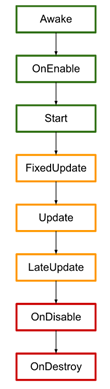
\includegraphics[scale=1]{img/ExecutionOrder.png}
	\caption{Orden de ejecución de los métodos habituales de un script}
	\label{fig:ordenEjecucion}
\end{figure}
\subsection{Modelos 3D}
Un modelo tridimensional de un videojuego se construye mediante una malla (\textit{mesh}). Esta malla está compuesta por vértices (puntos en el espacio) conectados entre sí generando aristas que crean caras poligonales, conformando así la superficie del modelo.

En un motor de videojuegos, los polígonos que forman estas caras son triángulos, ya que es el único polígono que genera un plano en el espacio, independiente de la posición de sus vértices. Cualquier otro polígono podría dar lugar a caras curvadas, lo que generaría errores cuando se rendericen e iluminen dichas caras.

Ello no implica que no se pueda trabajar con otro tipo de polígonos a la hora de modelar los objetos y personajes que se vayan a incluir en el videojuego, como ocurre en otros programas de modelado como Blender. De hecho, suele ser más conveniente utilizar cuadriláteros (\textit{quads}) cuando se crean los modelos del videojuego.
Sin embargo, cuando se importe la malla tridimensional al motor de videojuegos, este convertirá automáticamente todas las caras que la componen en triángulos (este proceso también es conocido como “triangular la malla”) para evitar cualquier tipo de complicación, artefactos inesperados o casos de error complejo cuando se renderiza el modelo.
\subsection{Battle Royale}
El término ``battle royale'' \cite{wiki:BattleRoyale} originalmente proviene de la película japonesa del año 2000 del mismo nombre que presenta un tema similar al de un último jugador en pie.
Más tarde se convertiría en término para referirse a un género específico de videojuegos en el que varios jugadores deben luchar entre ellos hasta que solamente quede un superviviente, que será el ganador de la partida.

Generalmente, una partida comienza distribuyendo de forma aleatoria una gran cantidad de jugadores en un gran mapa, normalmente entre 50 y 100, dependiendo de las dimensiones del mapa.

Se diferencia de los clásicos \textit{shooters} en que incorpora elementos de supervivencia, ya que los jugadores comienzan con un equipamiento nulo y tendrán que encontrar, dispersos por el mapa, cajas, armamento, armaduras, munición y otros elementos beneficiosos para el combate y la supervivencia.\\
Además, el equipamiento de los demás enemigos también puede ser saqueado cuando sean eliminados. Por lo tanto, durante la partida, los jugadores tratarán de equiparse lo mejor posible mientras evitan ser eliminados por otros jugadores.

Un punto clave en este género es que el mapa dispone de una “zona segura” que va disminuyendo su tamaño progresivamente a lo largo de la partida. Esto obliga a los jugadores supervivientes a permanecer en dicha zona, lo que hará que cada vez estén más cerca los unos de los otros y por tanto aumenta las posibilidades de que se encuentren. Los jugadores que se queden fuera de este área irán recibiendo daño incluso hasta ser eliminados si no consiguen entrar en la zona segura rápidamente.

La naturaleza aleatoria de la ubicación de los enemigos y los objetos, así como la reducción del área segura, hacen que el género battle royale sea ideal para desafiar a los jugadores a pensar, actuar rápidamente y mejorar sus estrategias durante el juego para ser el último en pie.

\capitulo{4}{Técnicas y herramientas} \label{TecnicasYHerramientas}

En este apartado se van a nombrar una serie de técnicas y herramientas que han sido de gran utilidad para llevaar a cabo el proyecto con un flujo de trabajo adecuado y eficiente.

\subsection{Blender}
Blender\cite{wiki:Blender} es una suite de creación 3D multiplataforma gratuita y de código abierto con la que se pueden crear modelos, visualizaciones y animaciones 3D. Su elemento principal de creación es la malla o \textit{mesh}, una estructura basada en polígonos editables y moldeables para construir los volúmenes deseados. Se pueden añadir, mover, eliminar o modificar tanto las caras como los vértices que las forman para crear los modelos tridimensionales con precisión.

Otros términos asociados a esta herramienta son los mapas UV, materiales, \textit{shaders} o los modificadores, importantes para obtener un flujo de trabajo adecuado en esta herramienta.

En este proyecto se ha utilizado Blender para crear varios modelos 3D incluidos en el juego, así como para texturizar algunos de ellos y crear animaciones para otros.

\subsection{Firebase Realtime Database}
Firebase Realtime Database \cite{wiki:Firebase} es una sistema gestor de base de datos (SGBD) NoSQL creado por Google. La base de datos se utiliza de manera remota en la nube y sincroniza los datos en tiempo real con todos los clientes conectados. Su funcionamiento se verá más en profundidad en el anexo C.

Es la base de datos elegida para el proyecto para que los usuarios puedan guardar su progreso en el juego, así como registrarse e iniciar sesión en él. 

\subsection{Github}
Github \cite{wiki:Github} es una plataforma para alojar proyectos software que utiliza el control de versiones \textit{Git}. Está pensada para que los desarrolladores puedan subir el código de sus aplicaciones a los llamados repositorios, lugares virtuales alojados en la nube donde poder almacenar cualquier tipo de archivo para mantener el proyecto a salvo y poder gestionarlo de manera más eficiente y segura.

El proyecto utiliza Github a modo de repositorio, como gestor de versiones para llevar un control sobre el mismo, y como gestor de tareas junto con la metodología \textit{Kanban}. Ha sido una herramienta esencial para llevar a cabo un desarrollo eficiente del proyecto.

\subsection{Latex}
Latex \cite{wiki:Latex} es un procesador de textos orientado a la redacción de textos de alta calidad tipográfica, como libros académicos, papers científicos, artículos y tesis. Esta herramienta, en conjunto con el editor online \textbf{\textit{Overleaf}} \cite{wiki:Overleaf}, se ha utilizado para redactar tanto la memoria como los anexos del proyecto. Al ser un procesador de textos un tanto particular y poco intuitivo en primera instancia, \textit{Overleaf} resulta de gran ayuda para visualizar el resultado en tiempo real de lo redactado en formato \textit{pdf}.

\subsection{Audacity}
Audacity \cite{wiki:Audacity} es un software de código abierto para la edición y mezcla de pistas de audio. En este proyecto, su uso se ha enfocado en la mezcla de diferentes sonidos para crear efectos interesantes y adecuados al juego. También se ha usado para el postprocesado de estas mezclas, añadiendo diferentes filtros o efectos y para ajustar su volumen.

\subsection{Illustrator}
Adobe Illustrator \cite{wiki:Illustrator} es un software de edición de imágenes centrado en la creación, edición y composición de gráficos vectoriales, muy útil para crear logotipos, iconos, y demás elementos formados a partir de vectores.
Este programa se ha utilizado en el proyecto para la creación de la mayoría de elementos de las interfaces del videojuego, como iconos, botones, paneles o fondos.

\subsection{Mixamo}
Adobe Mixamo \cite{wiki:Mixamo} es un software de servicio web dedicado a proporcionar modelos y animaciones 3D. Si bien dispone de modelos 3D de personajes en alta calidad, este programa se utiliza principalmente para agregar animaciones a modelos 3D humanoides de manera fácil. Para ello, utiliza técnicas de machine learning para dotar al modelo de un “esqueleto humano” a partir del cual crear las animaciones automáticamente.

Como se explica en el apartado “Aspectos relevantes del proyecto” \ref{Aspectos relevantes}, se ha utilizado esta herramienta para dotar de animaciones a los enemigos.

\subsection{Unity}
Unity 3D o simplemente Unity \cite{wiki:Unity}, es el motor de videojuegos empleado en el proyecto. Integra los diferentes componentes propios de un motor de videojuegos para gestionar aspectos como los gráficos, las físicas, la animación, la inteligencia artificial o el sonido. El lenguaje que utiliza para programar los \textit{scripts} es C\#.\\
Otras de sus características más destacadas son su amplio soporte a múltiples plataformas (PC, dispositivos móviles, consolas, realidad virtual, etc.), la gran comunidad de usuarios que posee, así como su amplia y detallada documentación.

Dentro de esta herramienta, existen diferentes elementos y conceptos que se utilizan de manera recurrente a lo largo del desarrollo del proyecto que son importantes de entender para comprender mejor este trabajo, y que son explicados más detalladamente en el apartado \ref{Conceptos teóricos}.

\subsection{Visual Studio}
Visual Studio \cite{wiki:VisualStudio} es el entorno de programación predeterminado para crear los scripts en Unity. Es un entorno de desarrollo integrado (IDE) muy completo, compatible con varios lenguajes como C\# y C++. Además, ofrece funciones de autocompletado y de depuración útiles para arreglar errores y carga automáticamente algunos de los \textit{namespaces} más utilizados en Unity. También permite crear diagramas de clases fácilmente a partir de las clases ya creadas.
\capitulo{5}{Aspectos relevantes del desarrollo del proyecto} \label{Aspectos relevantes}

En este apartado se trata de recopilar y detallarlos aspectos más interesantes que tuvieron lugar durante el desarrollo del proyecto y el porqué de algunas decisiones tomadas, así como las cuestiones y dificultades más destacables que surgieron y cómo se abordaron.

\section{Por qué Unity y no otro motor}
Durante la fase de planteamiento del proyecto, se tuvo que decidir qué motor de videojuegos se emplearía como base para el desarrollo del videojuego. Esta es una decisión clave, ya que sentará las bases del modo de trabajo del proyecto, es decir, que condicionará el tipo de cosas que se pueden hacer y cómo se hacen.

Dada la previa experiencia con Unity y Unreal Engine, el espectro de decisión se redujo a esos dos motores, que además son de los más populares y utilizados en la industria.No existe un motor mejor que otro, sino que, dependiendo del alcance y los objetivos del proyecto, será más conveniente utilizar uno u otro. 

Por lo tanto, tras una valoración de estos objetivos y plazos del proyecto, se decidió emplear el motor Unity. En términos generales, Unity es un motor de videojuegos más sencillo para desarrolladores principiantes, pero que no deja de ser potente para proyectos como el que se pretende desarrollar, y es por ello que es la opción escogida.

Los factores que hicieron decantar la balanza a su favor son los siguientes:
\begin{description}
\tightlist
	\item [Experiencia]: El alumno tenía experiencia previa en Unity, habiendo desarrollado algún pequeño proyecto en el pasado, a diferencia de Unreal Engine, con el que el contacto era más escaso, únicamente habiendo trasteado con sus funcionalidades de manera superficial. Esto hace que la curva de aprendizaje para poder desarrollar un proyecto de mayor magnitud como el que se presenta sea mucho menor.\\
	También permite dedicar más tiempo al proyecto en sí en lugar de destinarlo en aprender nuevas herramientas y modos de trabajo que el alumno tiene menos asentados. Esta familiaridad hace que el flujo de trabajo sea más sencillo y natural, consiguiendo un desarrollo más eficiente en todos los aspectos.
	\item [Programación]: En términos de programación, Unity utiliza el lenguaje C\#, mientras que Unreal usa C++ en conjunción con un sistema de programación visual denominado \textit{Blueprint}. C\# es un lenguaje más sencillo de aprender que C++ a ojos del alumno, ya que principalmente utiliza una metodología orientada a objetos, asemejándose en gran medida a otros lenguajes como Java, utilizado por el alumno durante su transcurso académico.
	\item [Comunidad de usuarios]: Uno de los aspectos más relevantes a la hora de decantarse por el motor Unity es la extensa comunidad de usuarios que tiene en comparación a Unreal Engine. Esto se traduce a que es mucho más sencillo encontrar tutoriales, foros, y, en general, soluciones que provienen de otros usuarios a dudas o errores que puedan surgir durante el desarrollo. Esto es esencial para poder generar un producto completo y no quedarse estancado en algún punto del proyecto, aún más teniendo en cuenta la escasa experiencia que posee el tutor con proyectos de este tipo.
	\item [Documentación]: En relación al anterior punto, la API de Unity cuenta con una documentación muy detallada en su página web, que de manera clara y estructurada, explica las clases, componentes y funciones del motor, con casos de ejemplo y un lenguaje natural que resulta de gran ayuda para poder usar el motor. Unreal Engine, por su parte, también tiene un manual online de uso, pero resulta más escueto y menos preciso.
	\item [Gráficos]: Otro aspecto importante es el aspecto gráfico. Unreal Engine ofrece una calidad de gráficos notablemente superior a Unity, con herramientas predefinidas como un sistema de iluminación preciso y realista, o varias opciones de postprocesado para conseguir un acabado más pulido.
	Unity, por su parte, tiene funcionalidades limitadas en el aspecto gráfico a la hora de crear una ambientación realista. Sin embargo, la estética definida para el proyecto es más caricaturesca que realista, siendo además uno de los objetivos del proyecto el crear un videojuego que pueda ser ejecutado en dispositivos de bajas prestaciones, algo difícil cuando se trata de imitar la realidad en un videojuego. Por lo tanto, dado que dichas herramientas no serían aprovechadas, Unity es la opción ideal para el tipo de proyecto que se trata.
\end{description}

\section{Por qué Firebase y no otro SGBD}
El objetivo central del proyecto no gira en torno a la base de datos del videojuego, sino que más bien es una extensión de este para que los usuarios puedan iniciar sesión y guardar datos simples, como su nombre de usuario y su experiencia.

Quizás, por las características del proyecto y la clase de datos que se almacenan, se podría pensar que una base de datos SQL, con el clásico modelo entidad-relación, hubiese sido la manera más adecuada de abordar esta cuestión.
Sin embargo, este modelo, aunque robusto, tiene algunas limitaciones que podrían ser clave si potencialmente se desea escalar el proyecto de algún modo. Quizás en un futuro de desee ampliar las funcionalidades de la base de datos para almacenar más elementos, crear un sistema más elaborado de objetos, incluyendo cosméticos para las armas, o, si finalmente se hace multijugador, poder responder a todas las peticiones del servidor de los jugadores online, entre otras muchas posibilidades.\\
Por esta razón, se consideró más adecuado integrar una base de datos no relacional (NoSQL), en vistas a futuro, para cumplimentar con el objetivo de extensibilidad del proyecto.

La ventaja principal de este modelo frente a las bases de datos SQL es su escalabilidad y su mayor velocidad. Son ideales para gestionar grandes volúmenes de datos cambiantes, que incluso pueden no estar estructurados, algo habitual en los videojuegos. Almacena los datos en forma de árbol en lenguaje JSON, lo que otorga una amplia flexibilidad, pudiéndose adaptar a las necesidades de cada proyecto más fácilmente que en los modelos relacionales. Además, tienen una arquitectura de escalado horizontal que permite gestionar la base de datos entre varias máquinas en caso de ser necesario.

En los videojuegos multijugador, es habitual ver este tipo de bases de datos, ya que necesitan gestionar grandes cantidades de datos de los jugadores en un tiempo muy reducido, a costa de en ocasiones perder el principio de integridad en las consultas de datos.

Con esto en mente, se buscó la manera más apropiada de integrar una base de datos NoSQL sencilla que se ajustase bien al proyecto sin crear complicaciones innecesarias.
Ante esta cuestión, las dos candidatas más apropiadas para cumplir esta tarea eran \textit{Mongo DB}, por recomendación del tutor, y \textit{Firebase Realtime Database}, por investigación propia.

Ambas comparten varias similitudes en funcionalidades, si bien\textit{MongoDB} es más potente desde la perspectiva de una base de datos, mientras que \textit{Firebase}ofrece más variedad de servicios integrados, como por ejemplo un sencillo y completo sistema de autenticación que permite seleccionar varios métodos de inicio de sesión para los usuarios de la aplicación, mostrados en la figura \ref{fig:Autenticación}.
\begin{figure}[h]
	\centering
	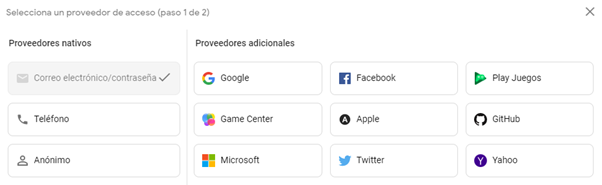
\includegraphics[scale=0.8]{img/DBAuthentication.png}
	\caption{Métodos de autenticación proporcionados por Firebase}
	\label{fig:Autenticación}
\end{figure}
Finalmente, considerando los requerimientos del proyecto y buscando un equilibrio entre funcionalidad y simplicidad, se ha acabado optando por \textbf{\textit{Firebase Realtime Database}} \cite{wiki:Firebase}. 
Uno de los aspectos clave de esta elección ha sido el hecho de que posee una guía detallada para integrar de forma sencilla la base de datos en Unity \cite{wiki:FirebaseWithUnity}, así como una consola web amigable. La guía de integración ha resultado de gran ayuda dada la inexperiencia del alumno integrando bases de datos en aplicaciones software, y las complicaciones que ello suele conllevar. 
De hecho, surgieron algunos problemas a la hora de configurar la base de datos, ya que en su integración en Unity, originalmente está pensada para funcionar sobre aplicaciones que se vayan a ejecutar en dispositivos móviles (Android e iOS). \\
Tras investigar el problema, no fue complicado adaptarla para hacerla funcionar sobre una aplicación de escritorio como la que se presenta. Simplemente se tuvo que crear una carpeta llamada StreamingAssets y añadir a ella el archivo google-services.json, descargado durante la configuración inicial de la base de datos de Firebase, pero renombrado como google-services-desktop.json.
En los apartados “Diseño de datos” y “Diseño arquitectonico” de los anexos, se detalla la configuración de la base de datos.

\section{Evolución del desarrollo}
En términos generales, la mayoría de sprints se entregaron en las fechas previstas. Sin embargo, en algunas fases del proyecto sucedieron ciertos contratiempos que retrasaron su desarrollo. El proyecto, si bien no tiene un desarrollo lineal, ya que se utiliz la metodología \textit{Kanban}, sí se puede dividir en cuatro grandes fases, dentro de las cuales se aplica dicha metodología, incluso pudiendo que se fusionen algunas fases entre ellas.                                      

La evolución de las fases y sus hechos más relevantes se detallan a continuación:

\subsection{Fase de planteamiento y definición}
Esta fase comprende desde el 1 de febrero de 2022 al 28 de febrero de 2022. Tiene como objetivo plantear el alcance del proyecto, sus requisitos básicos y la definición de los próximos sprints. Para definir de mejor manera el proyecto y sus características, se redacta un documento llamado \textit{Game Design Document} con el que se trata de cubrir varios puntos en relación al proyecto, tales como la definición concreta del proyecto, la descripción de su público objetivo, la temática, estética, tono y filosofía.

Un hecho remarcable durante el transcurso de esta fase fue que, en torno al 10 de febrero de 2022, tanto al tutor como al alumno se les propuso realizar el proyecto de manera conjunta con los integrantes de ITACA, el Centro de Innovación y Tecnología en Videojuegos y Comunicación Audiovisual de la Universidad de Burgos. Se valoró esta opción, pues podría ser beneficioso ampliar el alcance del proyecto e integrar más personas en su desarrollo para crear un mejor producto, más trabajado y pulido.

Durante algunas semanas se intentó concertar una reunión para valorar cómo se podría integrar la idea del alumno con la del resto de miembros del centro, así como la asignación de roles y tareas. Sin embargo, y pese a la insistencia tanto del alumno como del tutor, dicha reunión no llegó a darse, debido a asuntos internos de ITACA, principalmente a la falta de tiempo por la mudanza del departamento que se estaba produciendo durante esas fechas.

Estos hechos hicieron que la situación del proyecto quedase en el aire durante varias semanas, no siendo hasta el 2 de abril de 2022 que se decidió continuar con el proyecto de manera autónoma, ya que los primeros sprints relativos a las tareas de desarrollo se estaban retrasando demasiado.

Esto también hizo que el proyecto se tuviese que redefinir levemente, pues el alcance inicialmente propuesto sería demasiado ambicioso para realizarse en el tiempo restante. Concretamente, se tuvo que descartar la idea de que todos los modelos que se usasen en el videojuego fueran hechos desde cero por el alumno, teniendo que importar algunos modelos de forma externa, como las armas o los enemigos.

\subsection{Fase de implementación y desarrollo}
Esta fase se planteó inicialmente para que comprendiese desde el 1 de marzo de 2022 al 25 de mayo de 2022. En ella se implementa el proyecto en sí, incluyendo todo el desarrollo de las mecánicas, assets y demás elementos del videojuego. Es la fase que más tiempo requiere, ya que envuelve la parte más gruesa del proyecto y donde más errores y retrasos pueden surgir.

Como se ha mencionado, ante la espera de si el proyecto se integraría en un nuevo flujo de trabajo grupal, se decidió comenzar algunos sprints de tareas, tales como el Movimiento del jugador, el sistema de vida, el diseño del HUD o la programación básica de los enemigos.\\
Esta decisión permitió minimizar el retraso de los sprints y que la planificación temporal del proyecto se viese lo menos afectada posible, hasta finalmente llegar a ponerse al día en cuanto a plazos de tiempo y sprints.

En un proyecto de este tipo, con tantos elementos a tener en cuenta, es difícil calcular el tiempo que tomará una tarea en completarse. Hay aspectos que, en primera instancia pueden parecer sencillos de implementar, pero que a la hora de desarrollarlos no lo sean tanto. Puede que haya que investigar al respecto para corregir fallos, adaptarlo de alguna forma e integrarlos con el resto de elementos, o finalmente descartarlos si se complica demasiado su implementación y no es indispensable en el proyecto.

Por ejemplo, inicialmente había una tarea llamada ``previsualización de la trayectoria de las granadas'', que consistía en hacer que al pulsar la tecla de ``apuntar'' con una granada equipada, se visualizase la trayectoria que describiría la granada al ser lanzada. Se planteó como una tarea sencilla, incluida en un sprint de una semana de duración.
Sin embargo, resultó ser una mecánica más complicada de lo que parecía, ya que, en resumen, se debía crear una ''escena fantasma'' en la que, mediante iteraciones físicas, se averiguase dónde se encontraría la granada durante un lapso de tiempo determinado y así poder dibujar dicha trayectoria en la escena principal.\\
Tras varias investigaciones al respecto, se consiguió implementar este sistema, si bien el sprint se entregó dos días más tarde de lo previsto.

No obstante, tras varias pruebas, se observó que el sistema no funcionaba del todo como se esperaba, ya que en ocasiones no calculaba los rebotes con los demás elementos de la escena y sobre todo hacía que el rendimiento del videojuego disminuyese enormemente cuando estaba activo. Finalmente se decidió desechar la idea, ya que, en términos generales, era un elemento no esencial que generaba más problemas que ventajas al proyecto.

En parte, este tipo de situaciones son desfavorables porque hacen que ciertas partes del proyecto se retrasen, pero también son de gran utilidad para el desarrollador si aprende de ello. Es decir, puede servir para que, a la hora de definir tareas futuras, se prioricen aquellas mecánicas y elementos que aportan un valor más grande al producto final, ante aquellas tareas secundarias que, si bien pueden incluirse en los sprints siguientes, no deben alargarse demasiado para no lastrar al resto de tareas.

Otras veces, la solución a un error es sencilla, pero cuesta averiguar dónde está el error. Por ejemplo, durante el desarrollo del sistema que genera de manera procedural el mapa de juego, se comentó la línea de código que generaba el terreno. Al no haber terreno, los demás elementos nunca encontraban un punto sobre el que instanciarse, formándose un bucle infinito que congelaba el editor al momento de iniciarlo, sin poder ver la consola de errores y teniendo que reiniciar el programa. Esto hizo que el proyecto estuviese detenido dos días hasta que se encontró el punto de conflicto en el script correspondiente.

Situaciones como las descritas anteriormente son habituales durante esta fase de desarrollo, lo que hace que la metodología ágil \textit{Kanban} sea ideal para poder gestionar estos contratiempos, fallos de cálculo temporal, bugs y demás imprevistos que surgen a lo largo del proyecto.

Finalmente se pudo entregar todo el producto, aunque se alargó hasta el 6 de junio principalmente a causa de la complicada implementación del sistema de generación procedural del mapa.

\subsection{Fase de pulido y optimización}
Esta fase abarca desde el 26 de mayo de 2022 hasta el 8 de junio de 2022. En ella la actividad se centra en la resolución de errores que quedaron por resolver en la fase de desarrollo, así como en la optimización del código para evitar tener líneas innecesarias o scripts que no se usen. También se aprovecha para refactorizar, organizar y pulir variables y funciones dentro de los scripts para que su legibilidad y mantenimiento sean más eficientes. Además, se mejoran algunos recursos visuales y sonoros para que el llamado ``game feel'' y la experiencia de usuario sean tan agradables como sea posible, añadiendo por ejemplo música al juego o rediseñando el inventario y las barras de vida del jugador.

Se cumplieron los objetivos satisfactoriamente, pero la fase se alargó hasta el 15 de junio a causa del retraso en la fase anterior, así como a errores que surgieron al refactorizar algunos scripts, concretamente en el script ``PlayerInventory'', haciendo que las armas no se equiparan correctamente en el inventario.

\subsection{Fase de prueba y documentación}
Esta fase final termina el 3 de julio de 2022, y consiste en realizar los documentos de la memoria y completar los anexos con lo que no se haya incluido ya durante el transcurso del proyecto. En esta etapa también se comprueba que el producto se puede descargar y ejecutar correctamente en varios dispositivos de distintas características, y que esté listo para entregarse como un producto completo.

\section{Animaciones}
Un aspecto relevante a comentar es la forma en que se han realizado las animaciones de los diferentes elementos del videojuego, ya que no todas han sido creadas de la misma manera.

Las animaciones se encargan de dar dinamismo y realismo al juego, y se pueden clasificar en tres grupos, según la técnica utilizada para generarlas:
\begin{enumerate}
  \item \textbf{\textit{Animaciones manuales}}. El primer grupo corresponde a las animaciones que han sido creadas al estilo ``clásico'' o ``manual'', mediante la combinación de poses de los modelos en diferentes \textit{keyframes}, e interpolando dichas poses para crear una animación fluida.\\
  Se ha utilizado el propio motor de animación de Unity para ello, salvo en la caja de suministros, que se ha animado en el programa \textit{Blender}.
  
  Los elementos del videojuego que han sido animados con esta técnica son:
  \begin{enumerate}
  \item \textbf{\textit{Brazos y manos del jugador}}. Incluye animaciones como el movimiento de los dedos cuando el jugador no tiene ningún objeto agarrado, o desplazarse hacia abajo cuando el jugador salta.
  \item \textbf{\textit{Caja de suministros}}. Incluye el conjunto de animaciones que forman la apertura de la caja.
  \item \textbf{\textit{Desenfundado y recarga de armas}}. Todas las animaciones de recarga de las armas han sido creadas manualmente, una por una, adaptándose a la forma y el estilo del arma para crear animaciones únicas y visualmente atractivas.
  \begin{figure}[h]
	\centering
	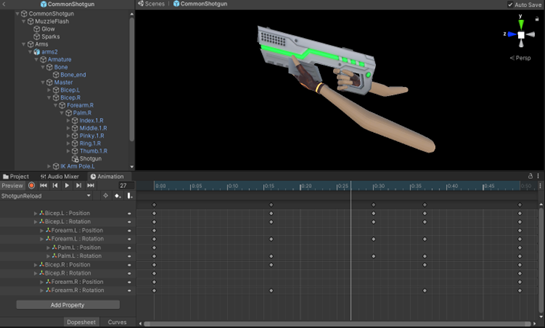
\includegraphics[scale=0.9]{img/ReloadAnimation.png}
	\caption{Proceso de animación de recarga de un arma}
	\label{fig:AnimaciónRecarga}
    \end{figure}
  \end{enumerate}
  \item \textbf{\textit{Animaciones creadas con Mixamo}}. Como se comentó en el apartado de ``Técnicas y herramientas''(\ref{TecnicasYHerramientas}), Mixamo es un software dedicado a crear animaciones a partir de modelos 3D humanoides.\\
  En el proyecto, se ha utilizado esta herramienta para animar todos los movimientos de los enemigos.
  
  \begin{figure}[h]
	\centering
	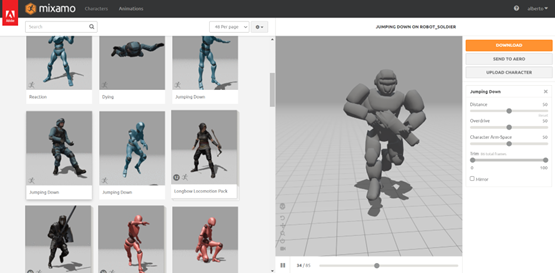
\includegraphics[scale=0.9]{img/MixamoScreenshot.png}
	\caption{Animación de modelos con Mixamo}
	\label{fig:AnimaciónMixamo}
    \end{figure}
    Mixamo, junto con Unity, proporcionan un flujo sencillo para generar animaciones:
    \begin{enumerate}
    \item Se arrastra el modelo 3 a Mixamo, y automáticamente creará unos ``huesos'', tomando en cuenta su volumen y sus proporciones.
    \item Después, se puede elegir entre una gran librería, la animación de movimiento o acción que se desea añadir al modelo.
    \item Una vez elegida la animación deseada, Mixamo animará el modelo a partir del ``esqueleto de huesos'' creado anteriormente. 
    \item Finalmente se exporta el archivo de la animación a Unity, donde se podrán ajustar algunos parámetros de la misma.
    \item Una vez se tengan todas las animaciones que se quieran añadir al modelo, se debe crear un \textit{Animator Controller}, que será el encargado de reproducir cada animación y cómo y cuándo se debe transicionar de unas a otras, como el que se ve en la figura \ref{fig:AnimatorController}.
    \end{enumerate}
    \begin{figure}[h]
	\centering
	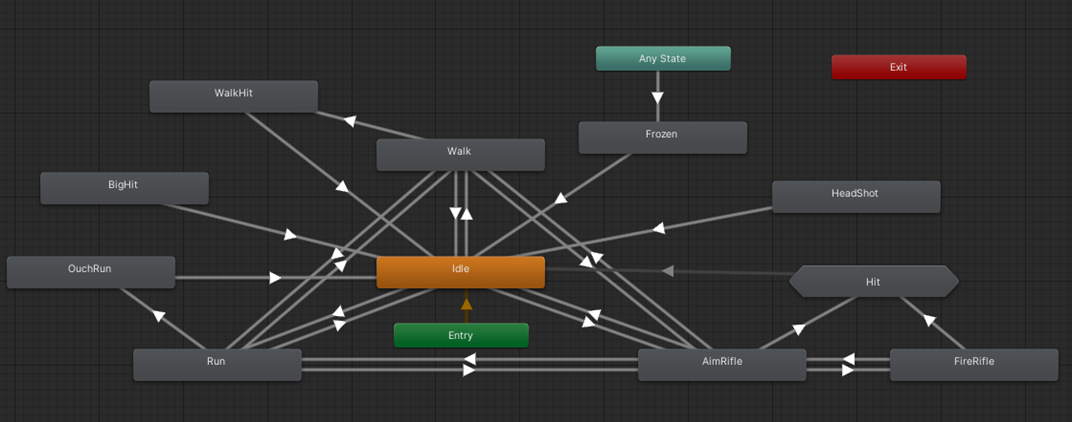
\includegraphics[scale=0.45]{img/AnimatorController.png}
	\caption{\textit{Animator Controller} de los enemigos con rifle y subfusil}
	\label{fig:AnimatorController}
    \end{figure}
    Un aspecto negativo de crear las animaciones en Mixamo es que, una vez hecha la importación en Unity, no se puede modificar directamente la animación, sino sólo algunas opciones básicas de configuración.\\ Además, no ofrece mucha personalización y está limitado a las animaciones de la su librería. Esto supuso que alguna animación no coincidiera bien con algunas armas de los enemigos, pero ajustando las opciones que ofrece, se pudieron minimizar los efectos no deseados.
    
    Gracias a esta herramienta se pudo agilizar la parte de animación del proyecto, ya que crear todas las animaciones de los enemigos manualmente hubiera llevado demasiado tiempo.
    \item \textbf{\textit{Animaciones procedurales}}. Se trata de animaciones creadas a través de código por medio de funciones matemáticas, así como de desplazamientos y rotaciones, en lugar de animar el modelo 3D directamente.
    
    Este tipo de animaciones son ideales para videojuegos, puesto que no están predefinidas, sino que se generan sobre la marcha, haciendo que no siempre sean iguales y aportando variedad, así como una mayor sensación de realismo y naturalidad. Además, al no estar ligadas a ningún modelo en concreto, son reutilizables en varios de ellos.\\
    Por contra, son más complicadas de implementar, ya que son poco intuitivas y se deben tener conocimientos de algunos conceptos matemáticos concretos.
    
    Esta técnica ha sido utilizada en los siguientes aspectos del videojuego:
    \begin{itemize}
    \tightlist
	\item \textbf{\textit{Movimiento pendular de cámara}}. Se utiliza la periodicidad propia de las funciones seno y coseno (ver figura \ref{fig:FuncionesSenoCoseno}) para generar el efecto pendular en la cámara cuando el jugador se mueve. Esto, unido a la velocidad del jugador para determinar la frecuencia y la amplitud, genera un movimiento periódico natural de balanceo y aporta más sensación de realismo al moverse.
	
	\begin{figure}[h]
	\centering
	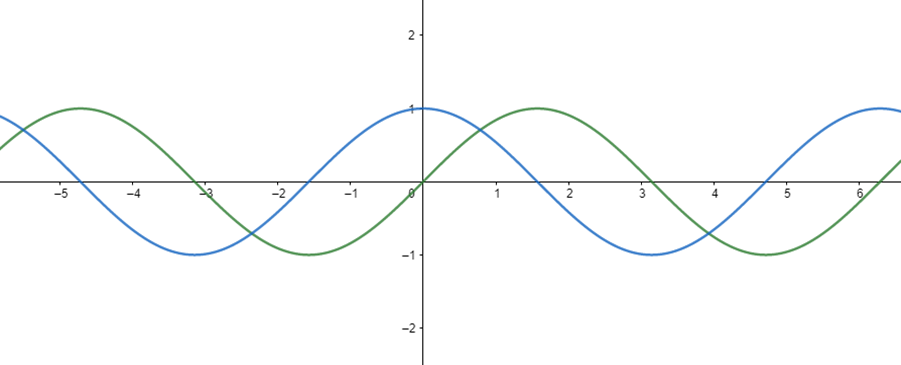
\includegraphics[scale=0.45]{img/sincos.png}
	\caption{funciones seno(verde) y coseno(azul)}
	\label{fig:FuncionesSenoCoseno}
    \end{figure}
    \item \textbf{\textit{Retroceso de las armas}}. El retroceso o \textit{recoil}bes un efecto propio de las armas de fuego que consiste en un movimiento provocado por la fuerza en sentido contrario al de la salida del proyectil. Para lograr este efecto, cada vez que se dispara el arma, se le aplica cierta rotación según los valores de ciertos atributos definidos en la clase \textit{Recoil}.
    
    Además de para aportar realismo, haciendo que las armas no se queden estáticas cuando se disparen, este efecto se utiliza en los videojuegos de estilo \textit{shooter} para evitar que el jugador siempre tenga una precisión total sobre las armas. El jugador debe adaptarse al retroceso de cada arma para poder disparar con mayor certeza, aportando un componente de reto y habilidad al hecho de acertar donde se pretende disparar.
	\end{itemize}
	Gracias a esta técnica, se puede reutilizar el mismo código para todas las armas que existen o vayan a existir en el juego, sin tener que animar cada arma una por una. Además, se obtiene un sistema completamente configurable para adaptar el retroceso de cada arma del juego de manera sencilla, modificando los valores de los parámetros que conforman el sistema.
	
	Este sistema ayuda a cumplir el objetivo de extensibilidad del videojuego, ya que se pueden añadir tantas armas como se desee, y su sistema de retroceso estará ya implementado.
\end{enumerate}

\section{Aleatoriedad}
Una de las características clave que se pretendía conseguir en este proyecto era crear un videojuego que con pocos elementos, tuviese una jugabilidad muy variada. Es decir, crear variaciones de los elementos que, en conjunto con la aleatoriedad, eviten que el jugador se aburra y siempre pueda encontrar algo diferente. Es por ello que se ha incorporado esta aleatoriedad y pluralidad en varios de los elementos del juego.

\subsection{Mapa procedural}
El elemento más destacable en cuanto a la aleatoriedad del juego es el mapa del juego donde se desarrolla la partida.\\
Para su diseño, inicialmente se planteó crear una composición estática en un programa de modelado 3D como Blender, con los diferentes modelos 3D disponibles, como edificios, cajas de suministros, decoración y demás elementos, para después exportar el mapa a Unity.

Sin embargo, más tarde se planteó otro método: Crear el mapa de manera procedural. Esta aproximación es más compleja de implementar en comparación a la alternativa inicial, que suele ser la habitual.\\
Finalmente se tomó a modo de reto personal el hecho de probar si sería viable utilizar este método, resolviendo los problemas que ello pudiera conllevar.\\
No fue una tarea sencilla, pero se consiguió implementar un sistema procedural de generación de mapas funcional para el proyecto.

La implementación de este sistema está contenida en la clase \textit{Spawner} y se construye con varias partes de manera secuencial:

\begin{enumerate}
  \item \textbf{\textit{Terreno base}}. Esta fue con diferencia la parte más complicada de implementar. El objetivo es generar mediante código un terreno que, lejos de ser plano y monótono, presente irregularidades a lo largo de toda su superficie. De esta manera, el jugador podrá caminar sobre él y sentir que se encuentra sobre un terreno interesante y verosímil, encontrándose con montañas y valles de distintos tamaños a su paso (Las montañas del fondo que rodean el mapa sí son siempre las mismas).
  
  Para lograrlo, se investigó la forma de poder llevar a cabo esta tarea, hasta que se encontró una lista de reproducción con varios tutoriales sobre la generación de terrenos aleatorios en Unity \cite{wiki:TerrainGeneration}, en los que se explican cómo poder generar de manera procedural este tipo de mallas en Unity gracias al llamado ruido de Perlin. Esta aproximación se tomó como base para lograr el objetivo, adecuándose al resto del proyecto.
  
  La forma en la que funciona la es la siguiente:
    \begin{enumerate}
    \item Primero se determinan las coordenadas ``x'' y ``z'' (plano horizontal) de cada vértice que formará la malla del terreno, según las dimensiones introducidas (figura \ref{fig:CoordenadasVertices}).
    
    \begin{figure}[h]
	\centering
	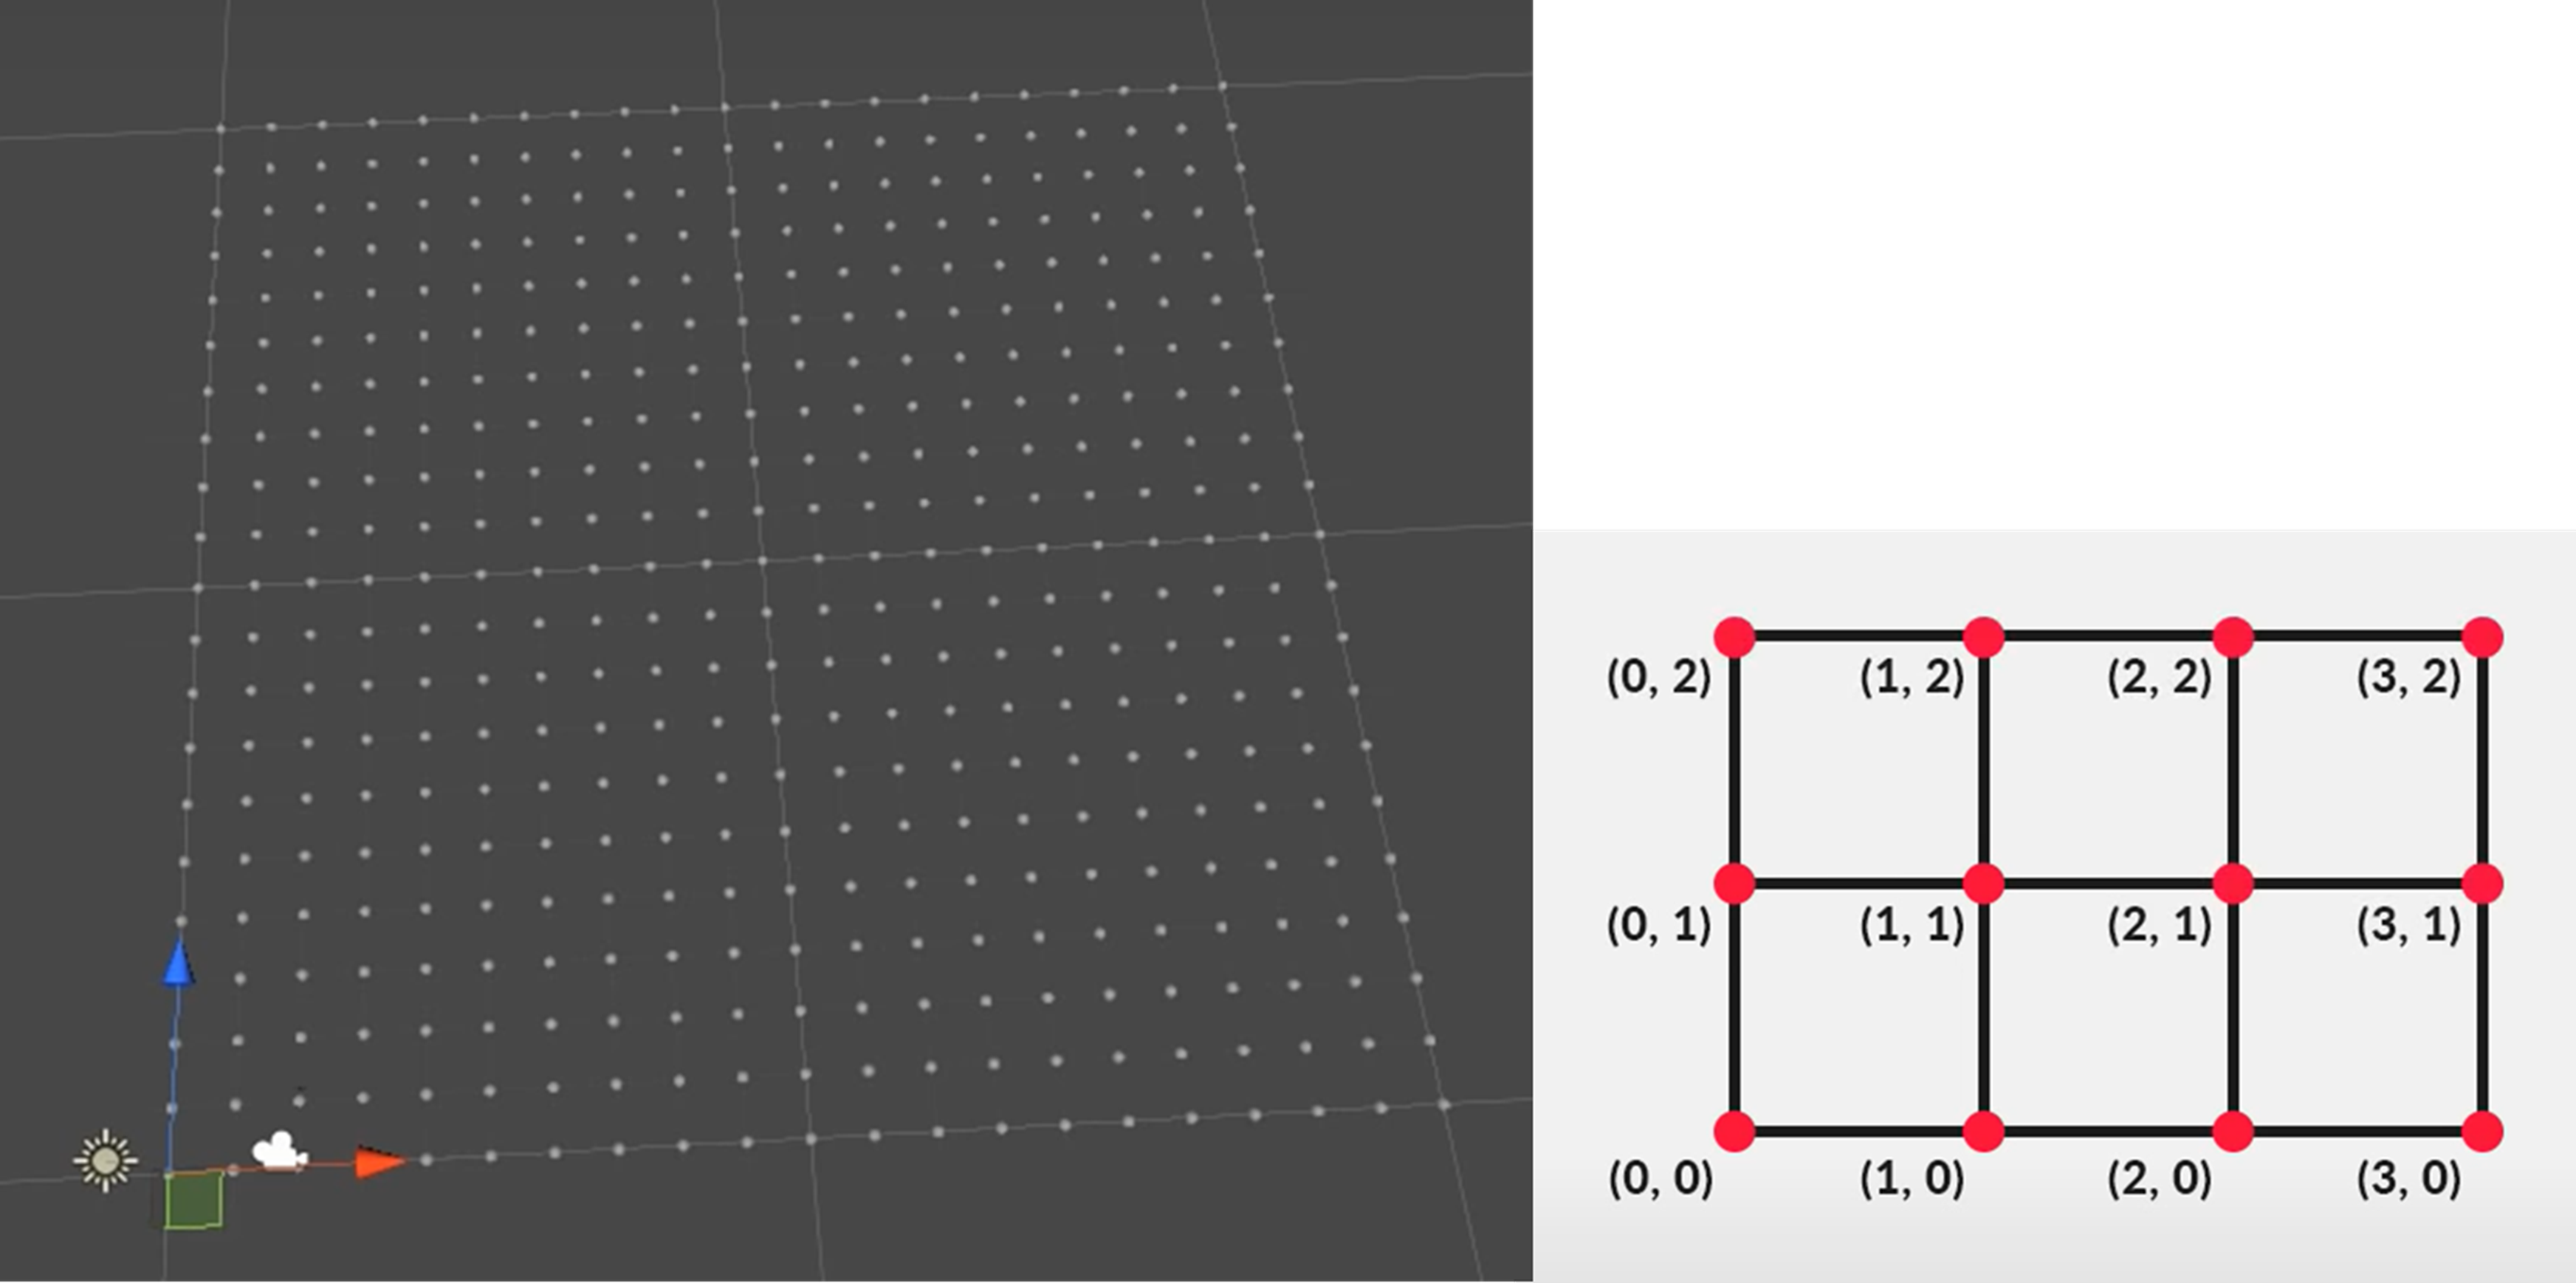
\includegraphics[scale=0.4]{img/verticesCoordinates.png}
	\caption{Representación de las coordenadas de los vértices}
	\label{fig:CoordenadasVertices}
    \end{figure}
    \item El siguiente paso es definir los triángulos que forman la malla, interconectando cada vértice con sus adyacentes de forma adecuada (figura \ref{fig:GeneracionMalla}).
    
    \begin{figure}[h]
	\centering
	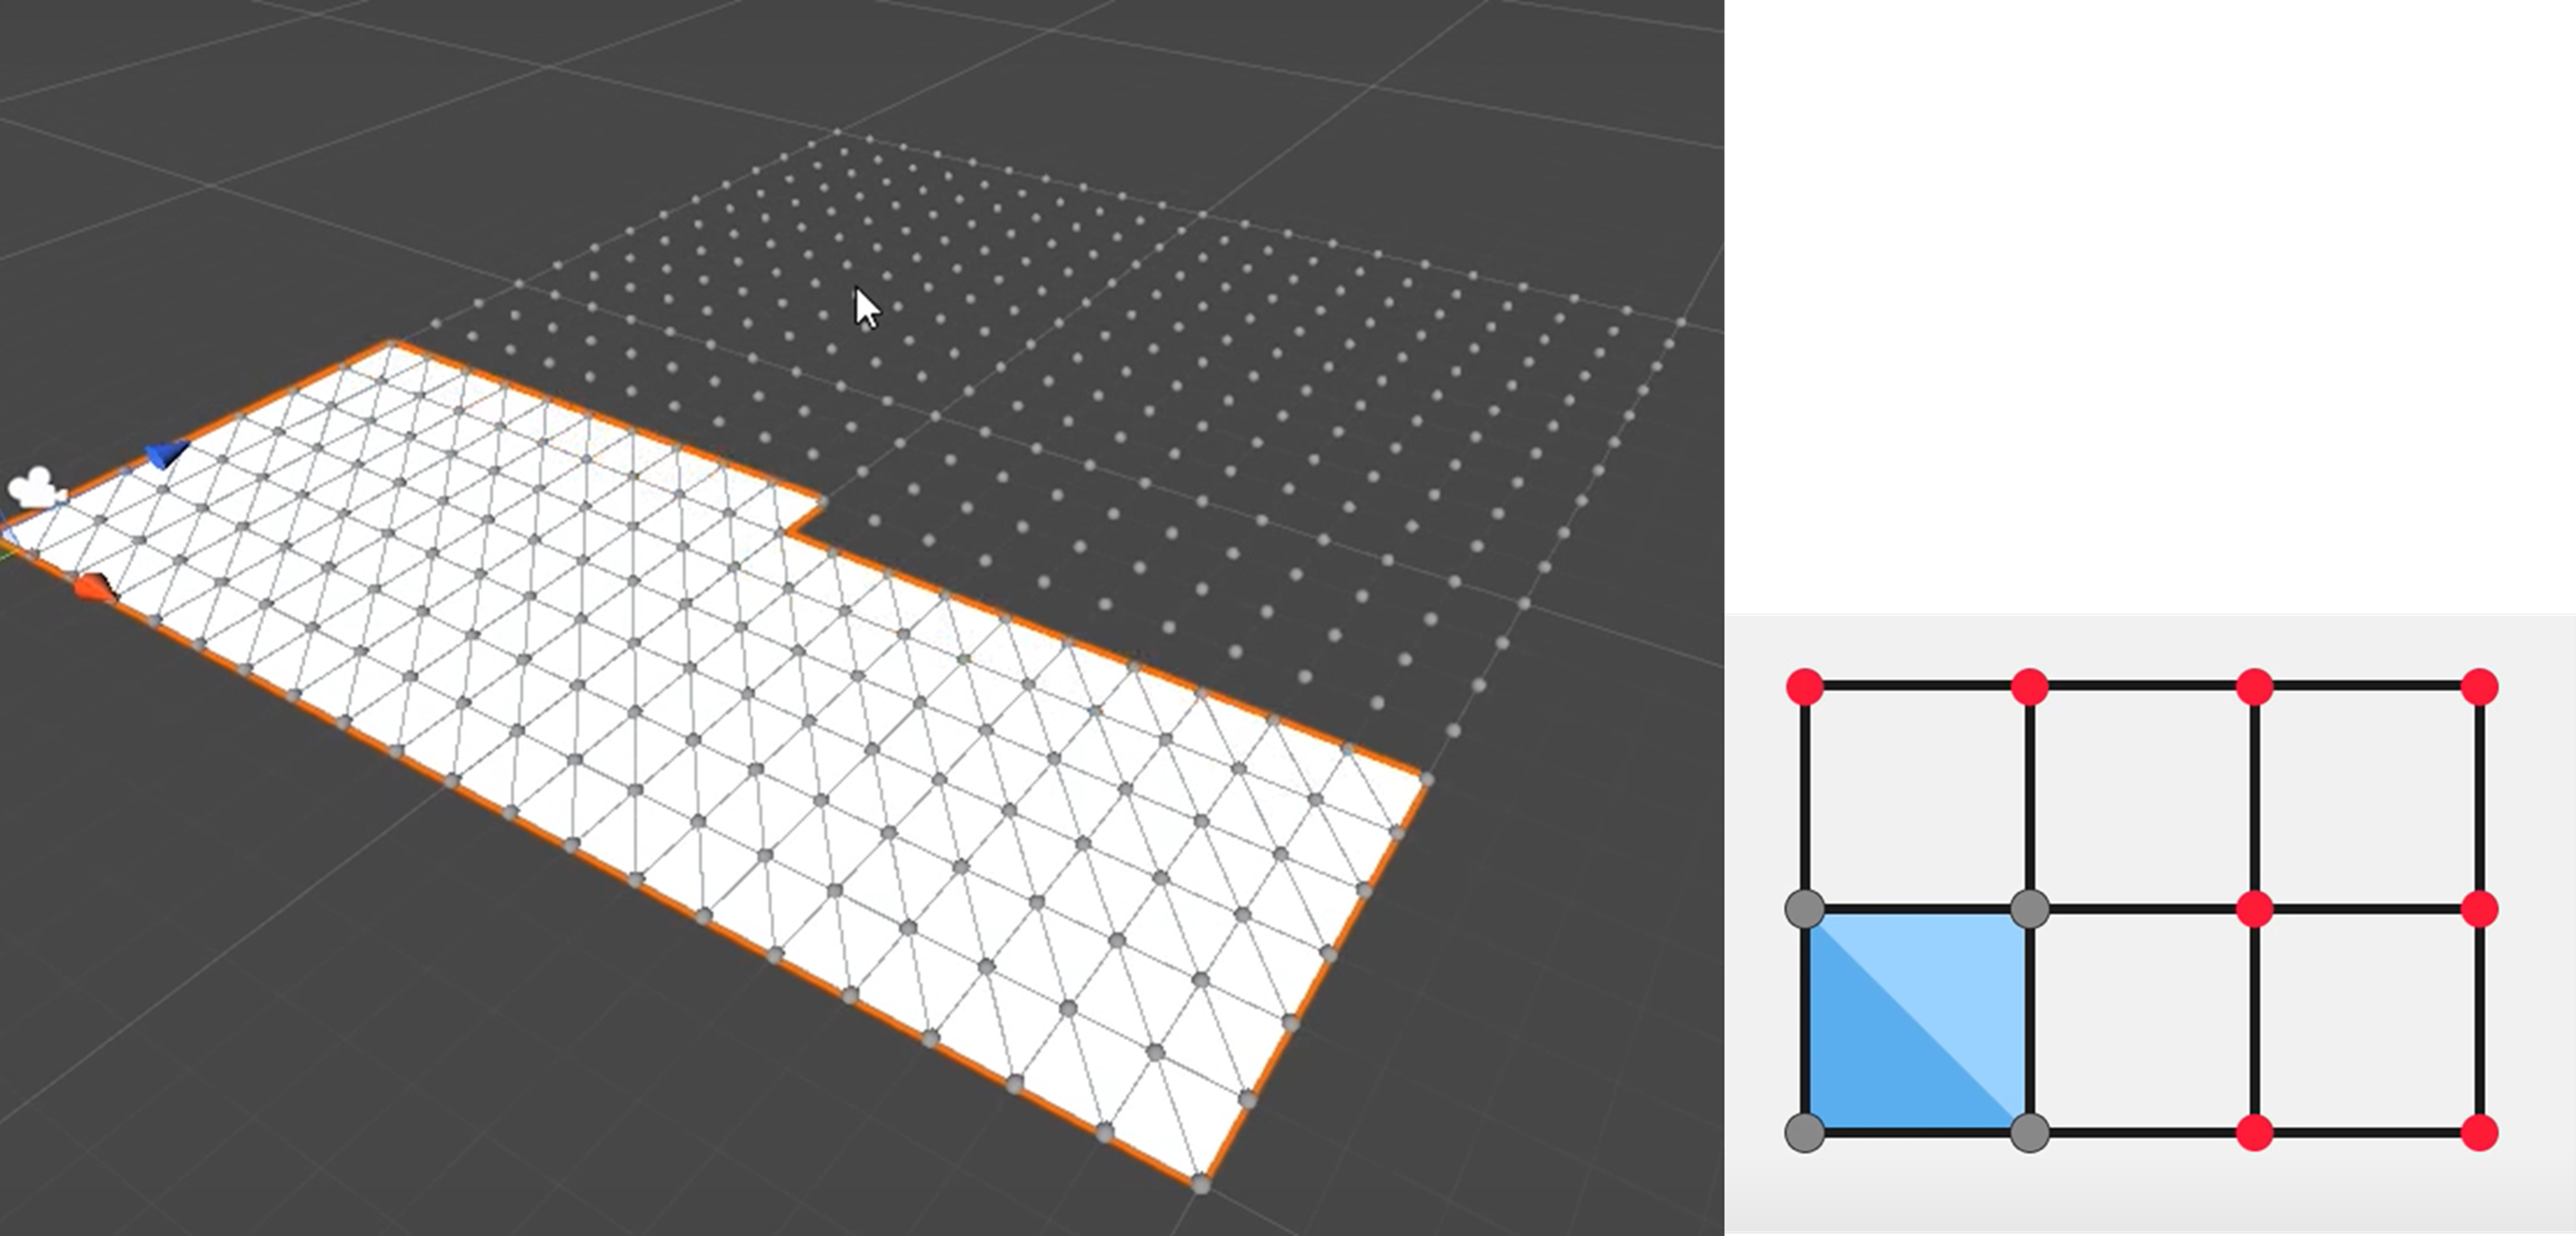
\includegraphics[scale=0.5]{img/MeshGeneration.png}
	\caption{Conexión de vértices para formar la malla}
	\label{fig:GeneracionMalla}
    \end{figure}
    \item Después se debe evitar que los vértices formen un plano como hasta ahora, sino que tengan diferentes alturas. No obstante, la altura de cada vértice no debe ser completamente aleatoria, ya que pueden formarse picos puntiagudos indeseados. En su lugar, se necesita que la altura de un vértice se vea condicionada por la altura de sus vértices vecinos, y así crear suaves colinas y valles.\\
    Para lograr esta tarea, se hace uso del ruido de Perlin o \textit{Perlin Noise} \cite{wiki:PerlinNoise}. El ruido de Perlin es una función matemática que utiliza la interpolación entre varios gradientes para generar un mapa 2D con diferentes valores pseudo-aleatorios pero sin perder cierta continuidad (figura \ref{fig:RuidoDePerlin}).
    
    \begin{figure}[h]
	\centering
	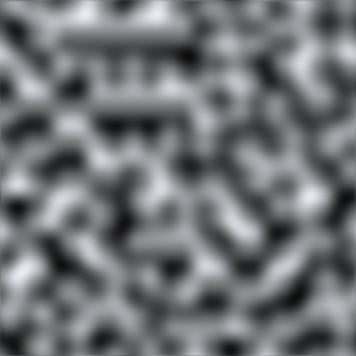
\includegraphics[scale=0.5]{img/PerlinNoise.png}
	\caption{Perlin Noise}
	\label{fig:RuidoDePerlin}
    \end{figure}
    A continuación se explicará cómo se utiliza el ruido de Perlin para determinar la altura de los vértices de la malla:
    \begin{enumerate}
    \item Lo primero que se hace es asignar a cada vértice un valor entre 0 y 1 dependiendo del color en la escala de grises del píxel correspondiente en la imagen de ruido de Perlin. Según este valor, al vértice le corresponderá una mayor o menor altura, siendo el color negro una altura de 0, mientras que el blanco representa la altura máxima de 1 (figura \ref{fig:PerlinPlano}).
    
    \begin{figure}[h]
	\centering
	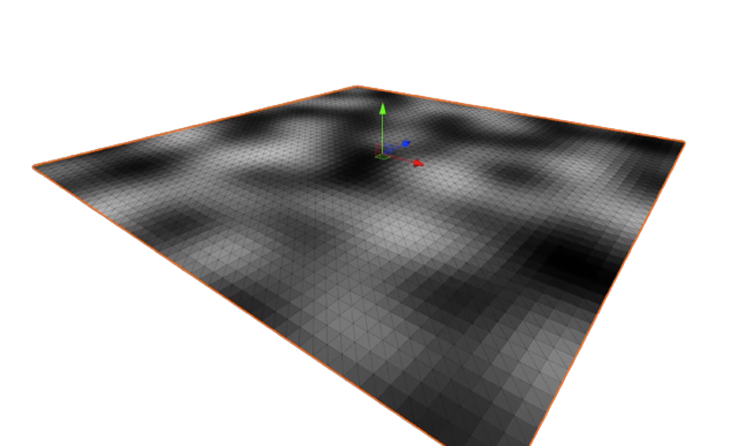
\includegraphics[scale=0.55]{img/PlainPerlin.png}
	\caption{Valores del Ruido de Perlin asignados a cada vértice}
	\label{fig:PerlinPlano}
    \end{figure}
    \item Posteriormente, se multiplica cada valor asignado por un número para generar la altura buscada(figura \ref{fig:PerlinConAltura}).
    
    \begin{figure}[h]
	\centering
	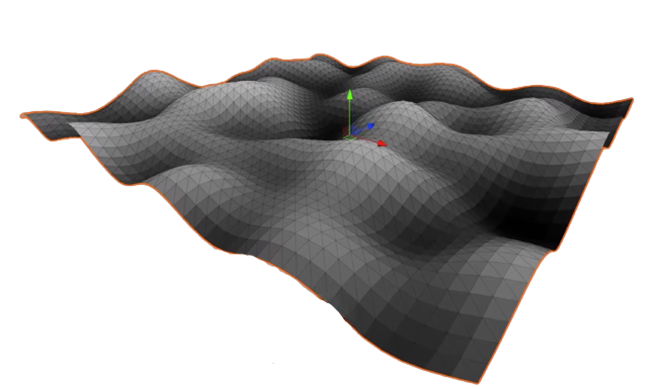
\includegraphics[scale=0.6]{img/HeightPerlin.png}
	\caption{vértices de la malla con altura según su valor de ruido de Perlin asignado}
	\label{fig:PerlinConAltura}
	\end{figure}
	\item El último paso del uso de esta función consiste en incrementar el componente aleatorio del terreno superponiendo varias capas de ruido de Perlin de diferente tamaño y amplitud. De esta forma se consigue generar un terreno más irregular e interesante.
    \end{enumerate}
    \item El último paso es colorear cada vértice según un gradiente de color determinado. Las zonas más bajas del terreno serán más oscuras, y las zonas más elevadas serán de un tono más claro. 
    \end{enumerate}
    La clase \textit{Spawner} escoge de manera aleatoria los valores de las funciones de Perlin superpuestas para que cada vez que se ejecute la aplicación, se genere una forma general de terreno diferente, con montañas y valles de diferente amplitud en cada caso. Además, también elige un gradiente de color de forma aleatoria para que el terreno tenga un tinte difetente en cada ocasión, como los que se pueden ver en la figura \ref{fig:TerrenosGenerados}.
    
    \begin{figure}[h]
	\centering
	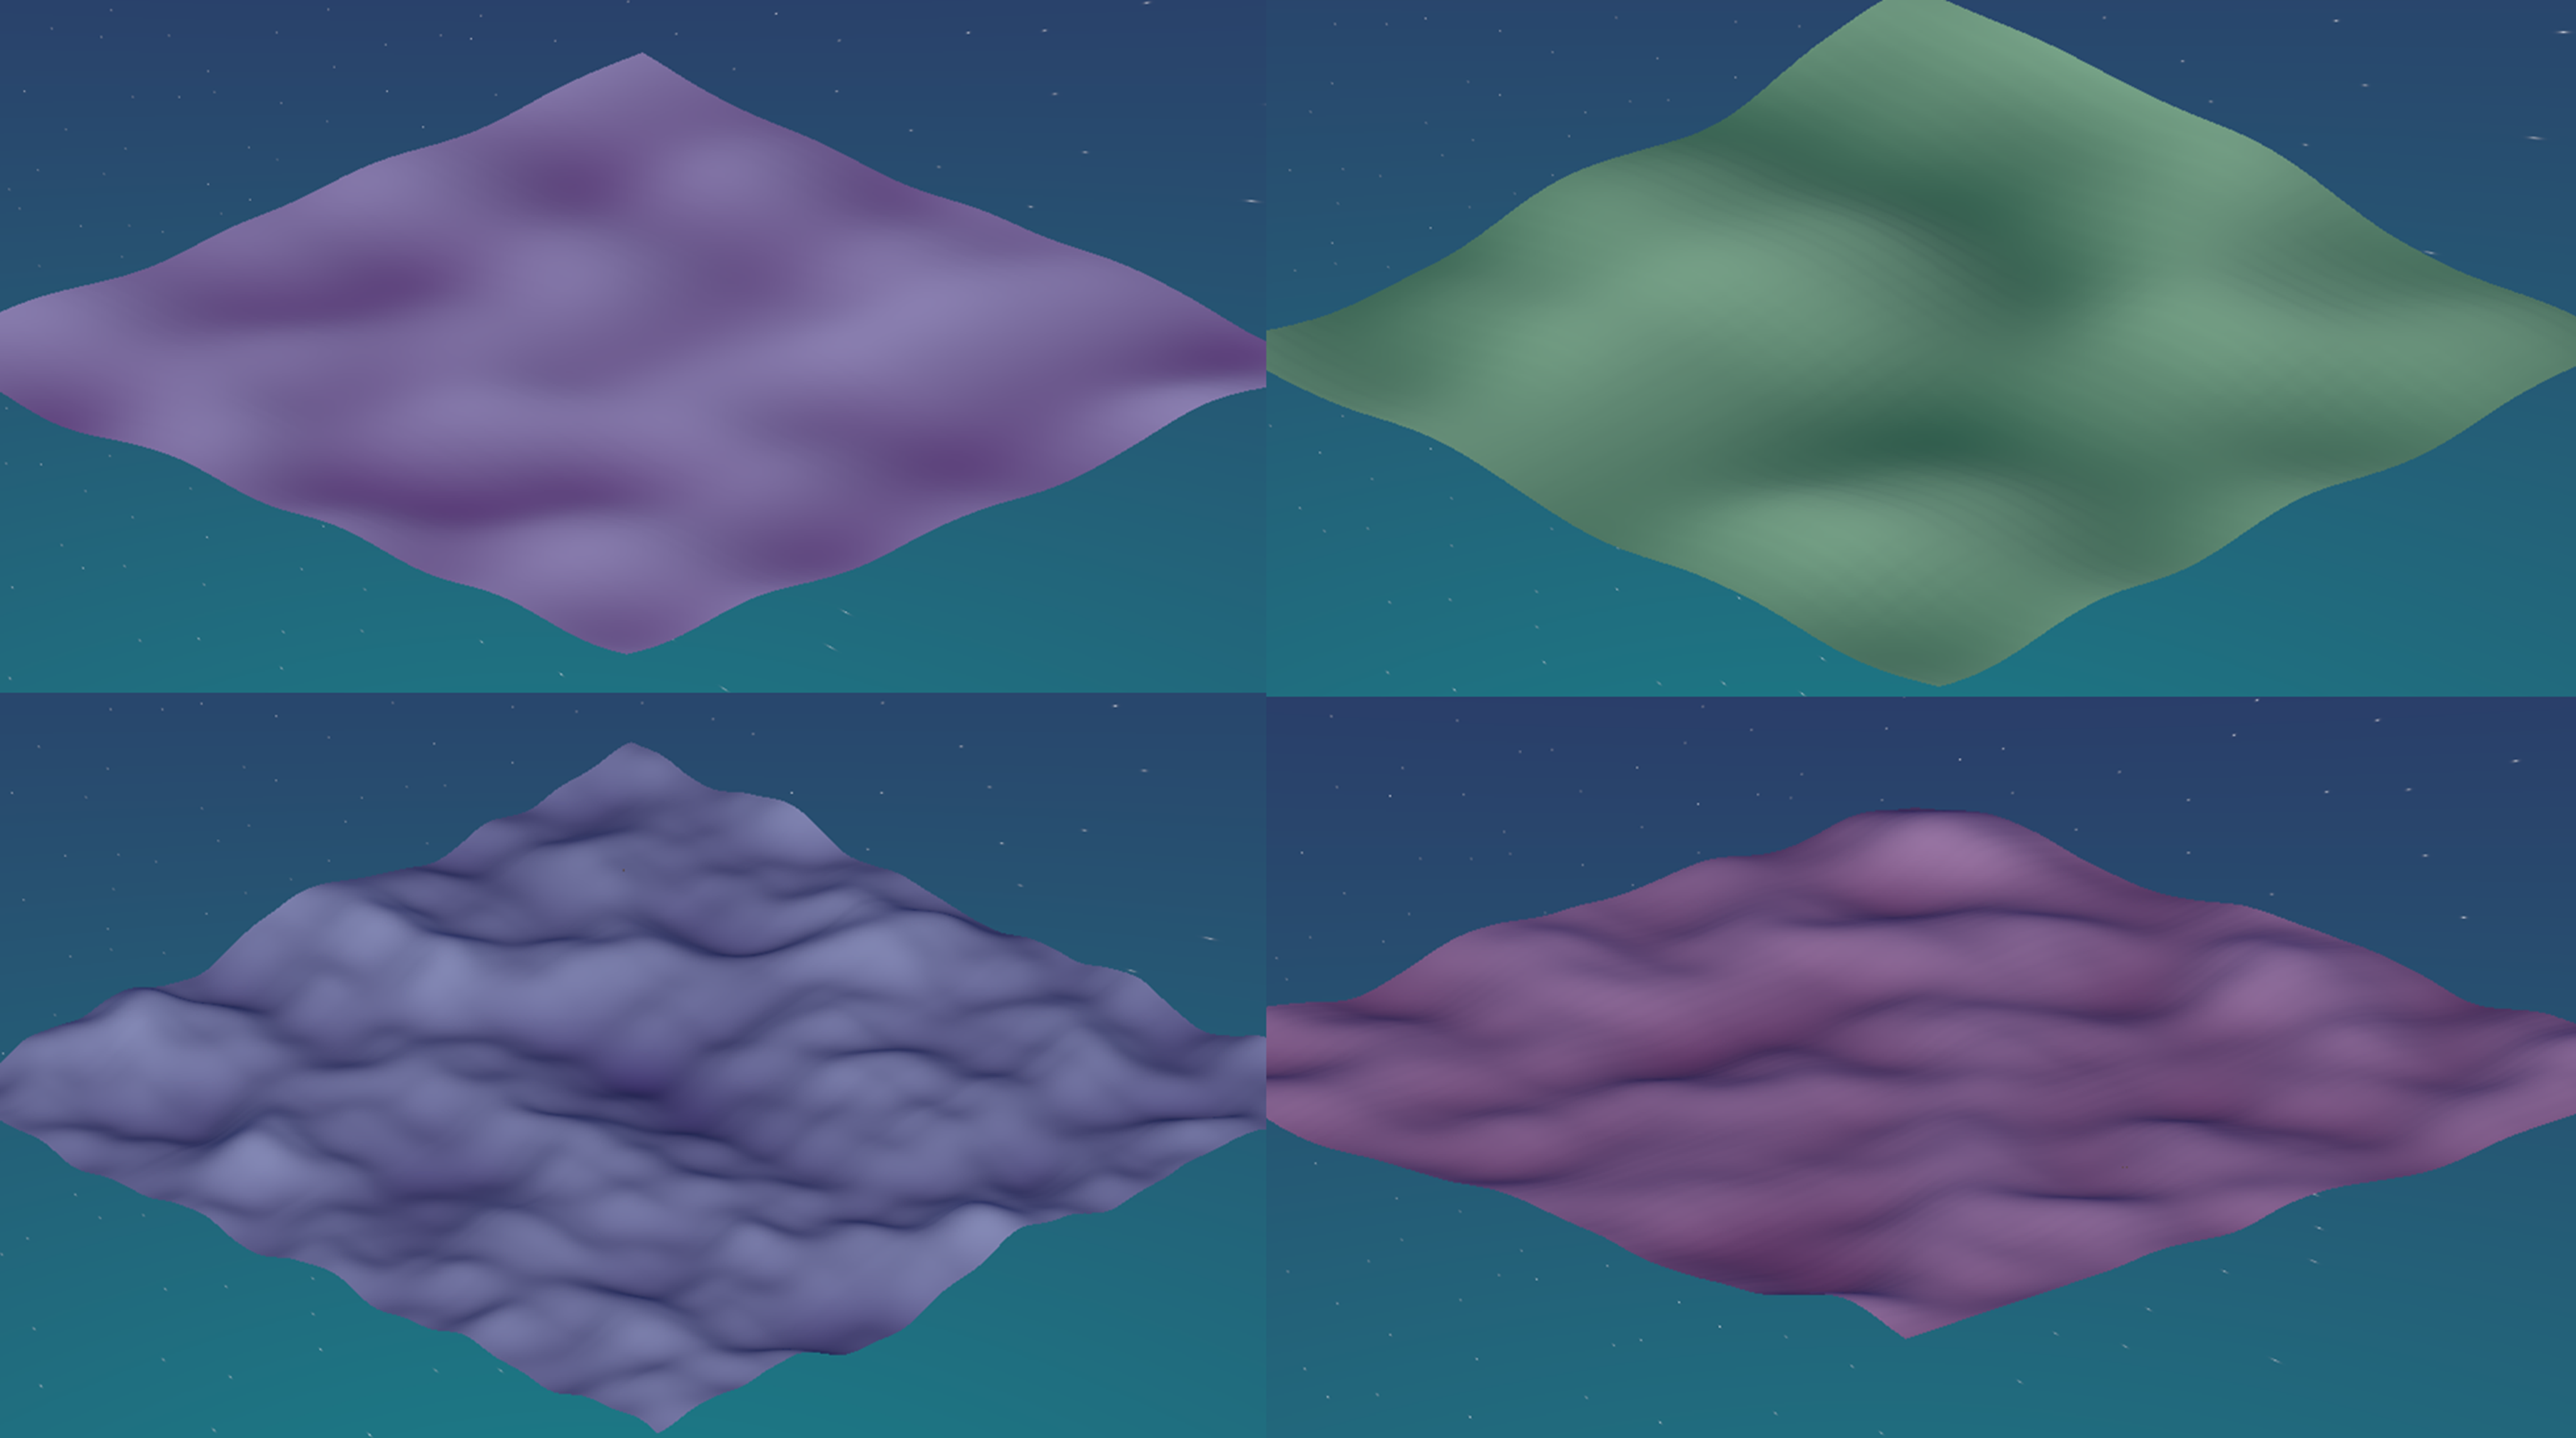
\includegraphics[scale=0.45]{img/GeneratedTerrains.png}
	\caption{Terrenos generados de manera procedural}
	\label{fig:TerrenosGenerados}
    \end{figure}
    \subsection{Problema con la superficie caminable}
    Un problema que surge al generar el terreno de esta manera es cómo hacer que los enemigos puedan caminar sobre él.
    
    Normalmente, cuando se dispone de un terreno predefinido, se puede hacer que las entidades no controladas por el jugador (\textit{Navmesh Agents})  tengan ``inteligencia'' para caminar debidamente por las superficies que se deseen. Esto se hace a través del componente \textit{NavMesh Surface}, que se añadirá a los gameobjects sobre los que se pretende que los enemigos puedan caminar. 
    
    Para construir la superficie caminable por los agentes, se ajustan unos valores del componente \textit{NavMesh Surface} desde el editor y se ``hornea'' (\textit{bake}) para que el motor defina dicha superficie.\\
    En el caso del terreno procedural, no se dispone de una superficie sobre la que ``hornear'' la superficie caminable desde el editor, ya que ni siquiera se conocerá qué forma tendrá el terreno hasta que se ejecute el juego.
    
    Unity no permite de forma nativa hacer estos cálculos dinámicos en tiempo de ejecución, por lo que, para poder conseguirlo, se ha tenido que importar un paquete experimental que aún está en desarrollo, llamado \textbf{\textit{NavMeshComponents}} \cite{wiki:NavMeshComponents}. Este contiene un conjunto de scripts con funcionalidades para calcular las zonas caminables de una malla en tiempo de ejecución de manera dinámica.
    
    Gracias a este paquete, y tras solucionar algunos errores, como que los enemigos se quedaban flotando a varios metros del terreno, se consiguió hacer que funcionase como se esperaba y los enemigos pudiesen deambular por el mapa (ver figura \ref{fig:SuperficieCaminable}).
    
    \begin{figure}[h]
	\centering
	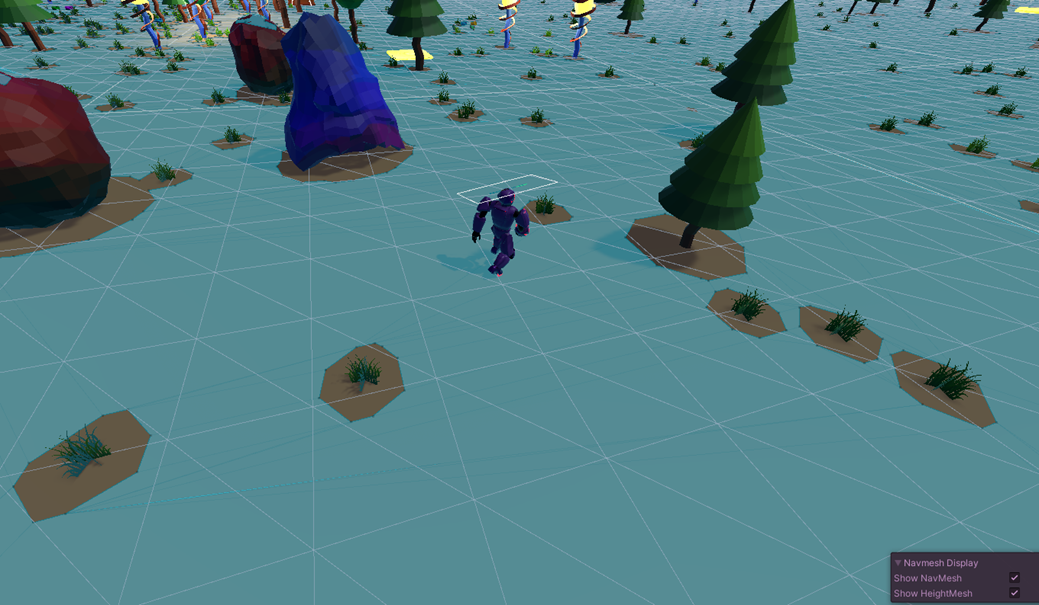
\includegraphics[scale=0.45]{img/NavMeshSurface.png}
	\caption{Superficie caminable (azul) calculada en tiempo de ejecución}
	\label{fig:SuperficieCaminable}
    \end{figure}
    No obstante, en la consola del editor siguen apareciendo advertencias y errores relacionados con el uso de estos scripts, mencionando que no está funcionando bien y que los componentes solamente funcionarán en el editor y no cuando el juego esté compilado. Sin embargo, tras compilar y exportar el juego se ha comprobado que también funciona correctamente, por lo que debe tratarse de algún \textit{bug} debido a que el paquete aún sigue en desarrollo.
    \item \textbf{\textit{Estructuras y edificios}}. La generación de edificios es un aspecto importante en la creación del mapa procedural del videojuego. Llenarán verticalmente el espacio, y harán que el terreno sea más interesante de explorar. Durante la partida, el jugador podrá interactuar con estos edificios, subiendo por ellos y encontrando cajas de suministros en zonas determinadas. Además, también servirán a modo de refugio o cobertura ante los ataques enemigos.
    
    La generación de estas estructuras funciona de la siguiente manera:
    \begin{enumerate}
    \item Se colocan puntos de referencia a lo largo de la zona donde se desean instanciar las estructuras.
    \item Una vez se genere el terreno base, se instanciará una estructura aleatoria de entre las disponibles, con un material aleatorio, en cada punto de referencia. Los rigidbodies de los edificios están definidos como \textit{kinematic}, lo que significa que no se pueden mover una vez instanciados. Esto se hace para evitar que las estructuras vuelquen por fuerzas externas y para poder asignarlas un \textit{mesh collider}, es decir, un collider que se adapte a su forma y volumen de manera precisa.\\
    Además, se impide que el terreno y los edificios puedan colisionar entre ellos para evitar errores con las físicas.
    
    \begin{figure}[h]
	\centering
	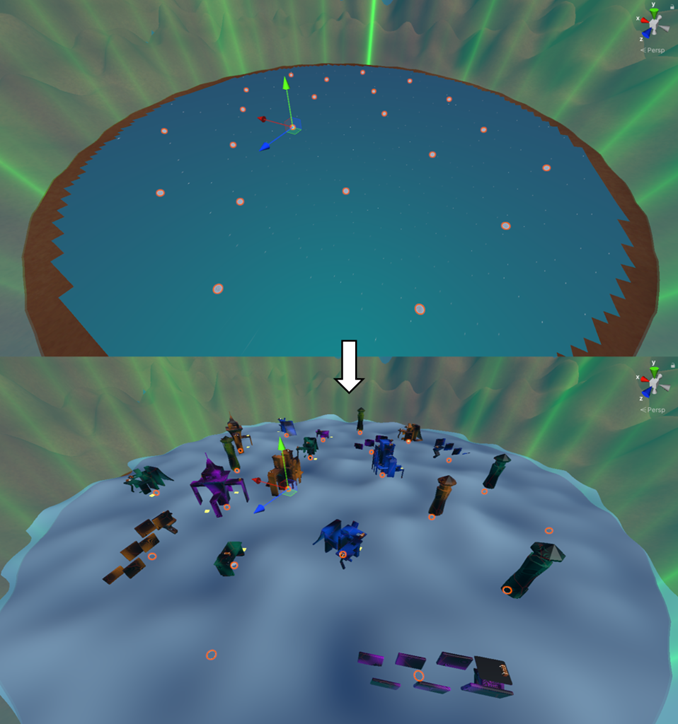
\includegraphics[scale=0.5]{img/BuildingsGenerator.png}
	\caption{Generación de edificios mediante puntos de referencia}
	\label{fig:GeneracionEdificios}
    \end{figure}
    \end{enumerate}
   Cabe destacar que, como el terreno tiene una altura que varía en cada punto, mientras que los edificios se instancian siempre en los mismos puntos, hay ocasiones que parte de los edificios queda oculta bajo el terreno.\\
   Esta característica puede verse como un fallo, pero, dada la forma desértica que genera el terreno, hace que los edificios parezcan haber sido enterrados bajo la arena, dando la sensación de un futuro postapocalíptico de un lugar abandonado y desértico, donde la naturaleza ha ganado la batalla contra las construcciones humanas.
    
    Además, no solo es algo visual, sino que, a nivel jugable, hace que en ocasiones las entradas principales de los edificios no sean accesibles porque se encuentran bajo el suelo. Esto hace que el jugador tenga que buscar otras maneras de alcanzar las zonas elevadas de las estructuras, ya sea saltando, utilizando plataformas de salto o corriendo por sus paredes.
    \item \textbf{\textit{Resto de elementos}}. El resto de elementos que se colocan sobre el mapa, como los enemigos, las cajas de suministros, las plataformas de salto, o los elementos decorativos como árboles, césped y rocas, se colocan de la misma manera.
    
    Para emplazar cada uno de ellos, se siguen estos pasos:
    \begin{enumerate}
    \item Se escoge un punto al azar a varios metros de altura sobre la zona que delimita el terreno.
    \item Se emite un \textit{raycast} hacia abajo hasta colisionar con algún gameobject.
    \item Si el gameobject con el que colisiona el rayo corresponde con el terreno, se instancia dicho elemento. En caso de ser cualquier otro tipo de elemento, se vuelve a comenzar en el primer paso. De esta forma, se evita instanciar unos elementos sobre otros, como que se genere un árbol encima de un edificio, por ejemplo.
    \item Se instancian tantos objetos de cada tipo como se indique en el objeto \textit{Spawner} de la escena.
    \begin{figure}[h]
	\centering
	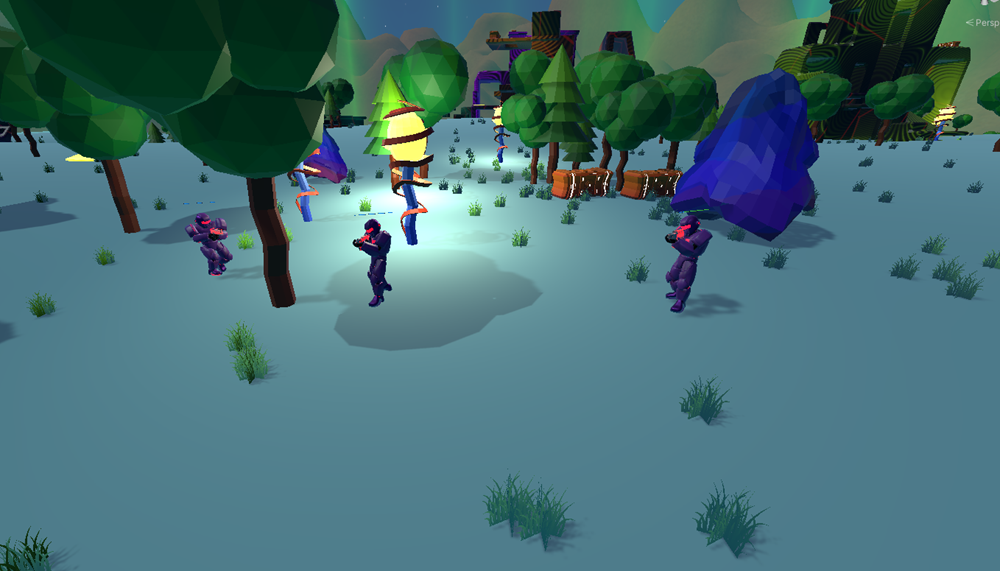
\includegraphics[scale=0.45]{img/ElementsGenerator.png}
	\caption{Varios elementos instanciados en el mapa}
	\label{fig:GeneracionElementos}
    \end{figure}
    \end{enumerate}
    
    Además, el \textit{Spawner} está diseñado para que sea sencillo modificar tanto el número de elementos que se instancian de cada tipo, como la clase de objetos que se instancian, además de poder cambiar los posibles colores del terreno y de los edificios, todo desde un mismo lugar (ver figura \ref{fig:AtributosGenerador}).

    \begin{figure}[h]
	\centering
	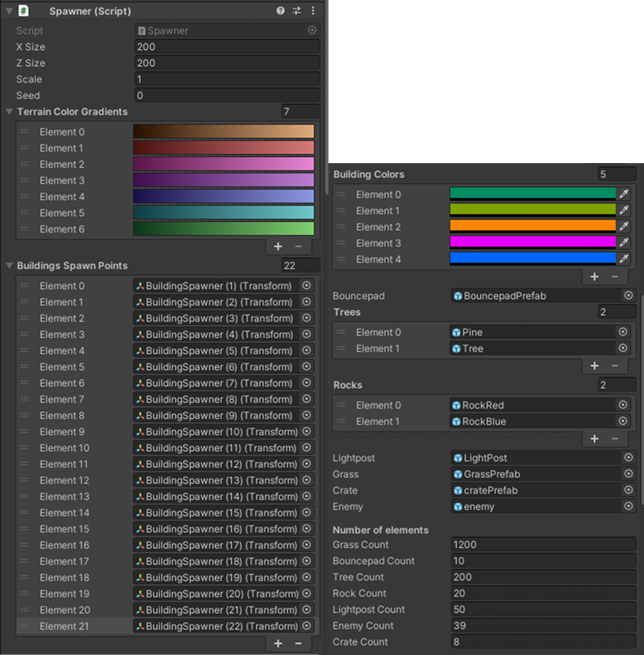
\includegraphics[scale=0.5]{img/SpawnerAttributes.png}
	\caption{Atributos y referencias expuestos de la clase \textit{Spawner}}
	\label{fig:AtributosGenerador}
    \end{figure}
\end{enumerate}

El objetivo principal de la implementación de esta técnica de generación procedural es obtener un sistema que genere un mapa diferente en cada partida. Cuando un jugador inicie una partida, se encontrará en un mapa nunca antes jugado por nadie más, es decir, que cada partida será única y diferente. Esto evita que el jugador se aprenda zonas del mapa que sean más ventajosas que otras, o que jugar una partida se sienta como algo monótono, potenciando en el videojuego el componente de exploración que se pretende conseguir.

\subsection{Armas, packs, rarezas y enemigos}
Otro hecho que ayuda a hacer que el juego no sea tan monótono es la variedad de \textbf{armas} disponibles en el videojuego. Existen cinco tipos de armas que tanto el jugador como los enemigos pueden usar, cuyas principales características se resumen en la tabla \ref{tab:armas}.
\begin{table}[t]
\begin{center}
\begin{tabular}{| c | c | c | c | c | c |}
\hline
\multicolumn{6}{ |c| }{Armas y sus estadísticas} \\ \hline
\textbf{Arma} & \textbf{Daño} & \textbf{Alcance} & \textbf{Recarga} & \textbf{Retroceso} & \textbf{Automática}\\ \hline
Pistola & Bajo & Corto-medio & Rápida & medio & No \\\hline
Escopeta & Alto & Corto & Rápida & alto & No \\\hline
Subfusil & Medio & Corto-medio & Rápida & alto & Sí \\\hline
Rifle de Asalto & Medio-alto & Medio-largo & Media & medio & Sí\\\hline
Francotirador & Alto & Largo & Lenta & medio & No\\\hline
\end{tabular}
\caption{Estadísticas de las armas}
\label{tab:armas}
\end{center}
\end{table}

Además, cada tipo de enemigo está asociado a un arma, por lo que habrá cinco tipos de enemigos, y las características de cada uno se definirán por el arma que utilice. Por ejemplo, un enemigo que use un francotirador podrá infligir daño al enemigo desde una larga distancia, mientras que otro que utilice una escopeta no podrá hacer daño al enemigo a menos que se acerque mucho a él (Figura \ref{fig:DosRobots}).

    \begin{figure}[h]
	\centering
	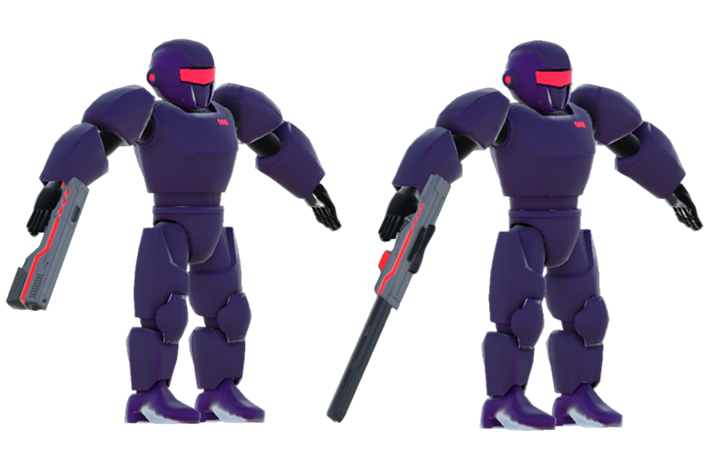
\includegraphics[scale=0.45]{img/RobotCouple.png}
	\caption{Ejemplo de diferentes tipos de enemigos}
	\label{fig:DosRobots}
    \end{figure}
En la parte del usuario, las armas que puede utilizar tienen cuatro posibles rarezas, cada una con características diferentes, recogidas en la tabla \ref{tab:rarezas}.
\begin{table}[t]
\begin{center}
\begin{tabular}{| c | c | c | c |}
\hline
\multicolumn{4}{ |c| }{Rarezas y estadísticas} \\ \hline
\textbf{Rareza} & \textbf{Color} & \textbf{Multiplicador} & \textbf{probabilidad}\\ \hline
Común & Verde & x1 & 50\% \\\hline
Rara & Azul & x2 & 30\% \\\hline
Épica & Morado & x3 & 15\% \\\hline
Legendaria & Amarillo & x4 & 5\% \\\hline
\end{tabular}
\caption{Estadísticas de las rarezas}
\label{tab:rarezas}
\end{center}
\end{table}

Además del multiplicador normal, si el disparo impacta sobre la cabeza del enemigo, se le infligirá el doble del daño habitual.

Esta tabla también es representativa, además de las armas, para los diferentes \textbf{packs de ayuda} que el jugador puede encontrar, tanto de munición (ver figura \ref{fig:Packs}), como de vida y de armadura. El multiplicador en cada caso hace referencia a algo distinto. En las armas, es el daño, en la munición, es el número de cargadores que se añaden, en el pack de vida, la cantidad de vida que cura, y en el caso del pack de armadura, la cantidad de armadura que recupera el jugador.

\begin{figure}[h]
	\centering
	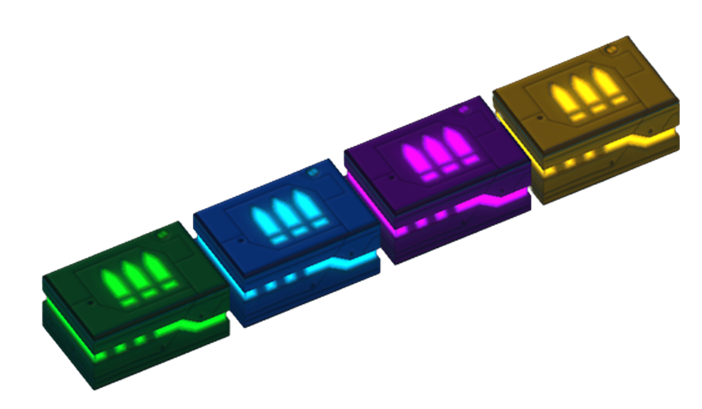
\includegraphics[scale=0.45]{img/Packs.png}
	\caption{Rarezas de los packs de munición}
	\label{fig:Packs}
    \end{figure}
Toda esta combinación de elementos hace que el juego aumente su grado de aleatoriedad para que el juego sea más variado y en definitiva, más divertido de jugar.

\section{Desarrollo de modelos 3D propios}
Un aspecto relevante a destacar del desarrollo es el hecho de que una sola persona ha desarrollado el videojuego por completo. Esto sumado a que el plazo para realizarlo es limitado y que los conocimientos de las herramientas y técnicas usadas era limitado, supone que el proyecto sea un ambicioso reto multidisciplinar a muchos niveles.

Una de estas disciplinas es el proceso de creación de modelos 3D propios, cuyo desarrollo puede ser de gran interés. En concreto, los modelos creados enteramente por el alumno son los que se enumeran a continuación, y se pueden visualizar en la figura \ref{fig:Modelos3D}.
\begin{itemize}
    \item Brazos y manos del jugador
    \item Caja de suministros
    \item Árboles
    \item Rocas
    \item Postes de luz
    \item Edificios y estructuras
    \item Plataforma de salto
    \item Nube tóxica
    \item Montañas
    \item Mirillas y otros elementos para modificar las armas
\end{itemize}

\begin{figure}[h]
	\centering
	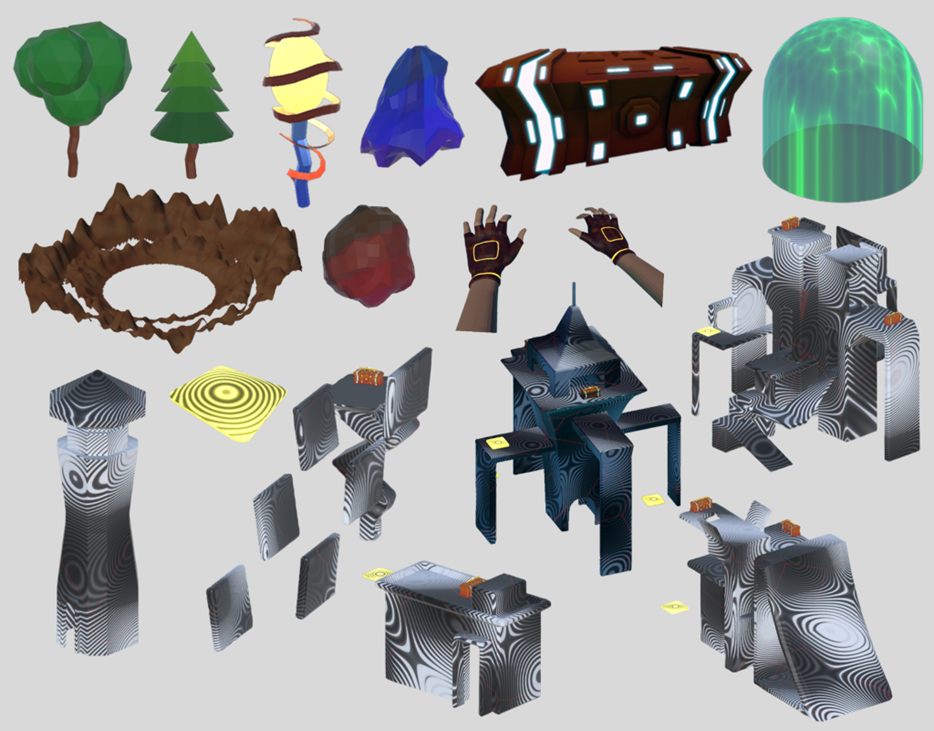
\includegraphics[scale=0.45]{img/3dmodels.png}
	\caption{Algunos de los modelos creados por el alumno}
	\label{fig:Modelos3D}
    \end{figure}
Todos estos objetos se han modelado en el programa \textit{Blender}, que también se ha usado para añadir materiales y texturas a cada uno de ellos. El proceso seguido para crear y texturizar un modelo se puede resumir en los siguientes pasos:
\begin{enumerate}
    \item Crear el \textbf{modelo} y el material deseado de Blender (ver figura \ref{fig:modeloManos}).
    \begin{figure}[h]
	\centering
	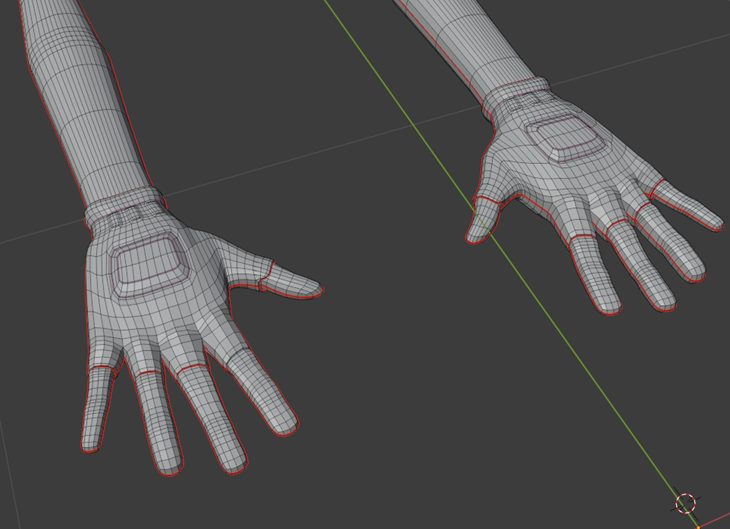
\includegraphics[scale=0.4]{img/ArmsModel.png}
	\caption{Modelo de las manos creado en \textit{Blender}}
	\label{fig:modeloManos}
    \end{figure}
    \item Generar un mapa de UV (\textbf{\textit{UV map}}) para el modelo. Este es una representación en dos dimensiones de cada punto del modelo 3D para poder asignar colores y texturas al modelo.
    \item ``Hornear'' (\textbf{\textit{bake}}) las texturas del modelo, es decir, a partir del mapa UV del modelo, generar distintas imágenes que representen el color, rugosidad, las zonas emisivas y demás propiedades que se deseen añadir al modelo.
    \begin{figure}[h]
	\centering
	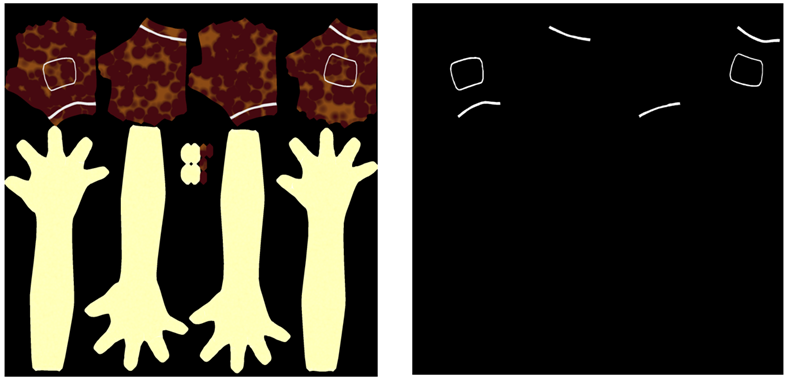
\includegraphics[scale=0.4]{img/ArmsTextures.png}
	\caption{Texturas de color (izquierda) y de emisión (derecha)}
	\label{fig:texturasManos}
    \end{figure}
    \item En caso de que el modelo necesite animarse, se le debe asignar un conjunto de \textbf{huesos} en los elementos móviles (ver figura \ref{fig:HuesosManos}).
    \begin{figure}[h]
	\centering
	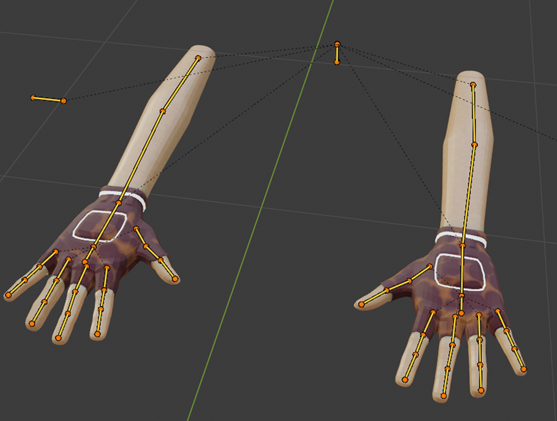
\includegraphics[scale=0.4]{img/ArmsBones.png}
	\caption{Esqueleto asignado al modelo para animarlo}
	\label{fig:HuesosManos}
    \end{figure}
    \item \textbf{Importar} el modelo en Unity
    \item Crear un \textbf{material} con las texturas generadas (ver figura \ref{fig:MaterialManos}).
    \begin{figure}[h]
	\centering
	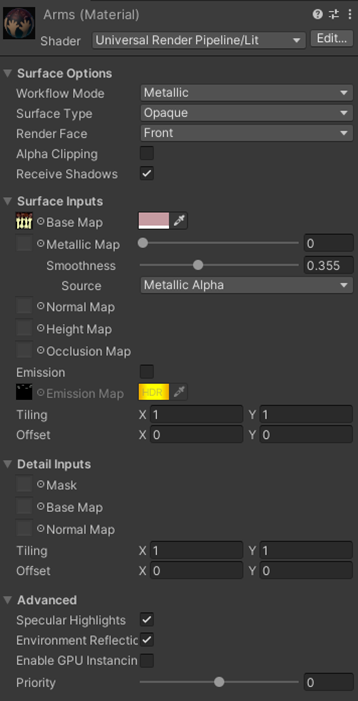
\includegraphics[scale=0.45]{img/ArmsMaterial.png}
	\caption{Material creado para el modelo de las manos}
	\label{fig:MaterialManos}
    \end{figure}
    \item \textbf{Asignar} el material al modelo terminar de tenerlo preparado para utilizarse. (ver figura \ref{fig:ManosFinal}).
    \begin{figure}[h]
	\centering
	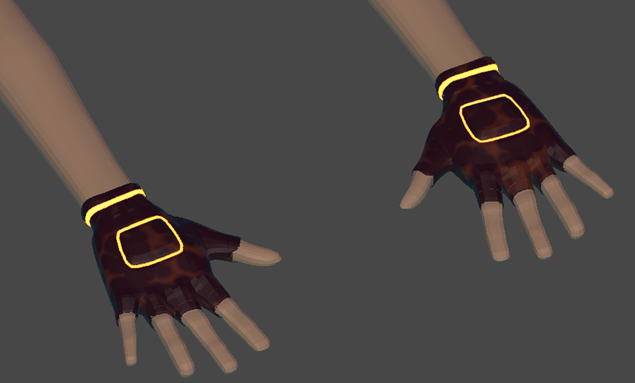
\includegraphics[scale=0.4]{img/ArmsFinal.png}
	\caption{Modelo texturizado final en Unity}
	\label{fig:ManosFinal}
    \end{figure}
    De esta manera se tendría el modelo listo para empezar a añadirle diferentes componentes, crear animaciones o lo que se necesite.
    
    En casos especiales, como el de la nube tóxica, en lugar de asignarles un material compuesto por texturas, como se hace habitualmente, se le asigna un material que utiliza un \textit{shader} personalizado especial para que pueda tener efectos de movimiento.
\end{enumerate}
\section{Etiquetas}
Un elemento cuyo diseño ha cambiado a lo largo del desarrollo es la etiqueta de información que aparece cuando el jugador observa un objeto con el que se puede interactuar.\\
Al principio se diseñó una etiqueta diferente y personalizada para cada objeto. Sin embargo, esto no respondía bien al objetivo de extensibilidad, ya que cada vez que se añadía un objeto se debía crear una etiqueta nueva, generando más archivos y ocupando más espacio.\\
Por ello, se desechó esta implementación, y en su lugar, tras varios intentos, se consiguió crear de un único prefab que sirviese para todas las etiquetas de información del juego.
\begin{figure}[h]
	\centering
	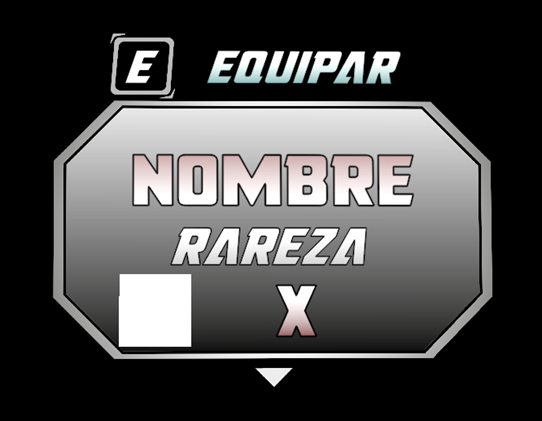
\includegraphics[scale=0.4]{img/LabelEmpty.png}
	\caption{Plantilla de las etiquetas de objeto}
	\label{fig:PlantillaEtiqueta}
    \end{figure}
La etiqueta se divide en varios campos: Un nombre para el objeto, el tipo o rareza que tiene y su estadística más relevante, junto a un icono representativo. Además tendrá un color en función de la rareza o tipo del objeto Ver figura \ref{fig:PlantillaEtiqueta}).
Jugando con estos campos se podrá crear una etiqueta personalizada para cada objeto, de forma que cada vez que se quiera generar una etiqueta desde el GameManager, se deberán pasar como parámetros los diferentes valores de estos campos para que se pueda instanciar correctamente.

Por ejemplo, cuando se quiera crear la etiqueta correspondiente a un subfusil raro, se rellena el nombre con el valor ``subfusil'', la rareza con ``raro'', la estadística más relevante es el daño por segundo que hace (100), y el icono para representarlo es una especie de impacto de bala. Si, por el contrario, se quiere generar la etiqueta para un pack de vida épico, el nombre ahora sería ``botiquín'', la rareza sería``épico'' y la estadística más relevante es la cantidad de vida que cura al jugador, junto a un icono de una cruz verde para representar el concepto de salud (ver figura \ref{fig:EjemplosEtiqueta}).
\begin{figure}[h]
	\centering
	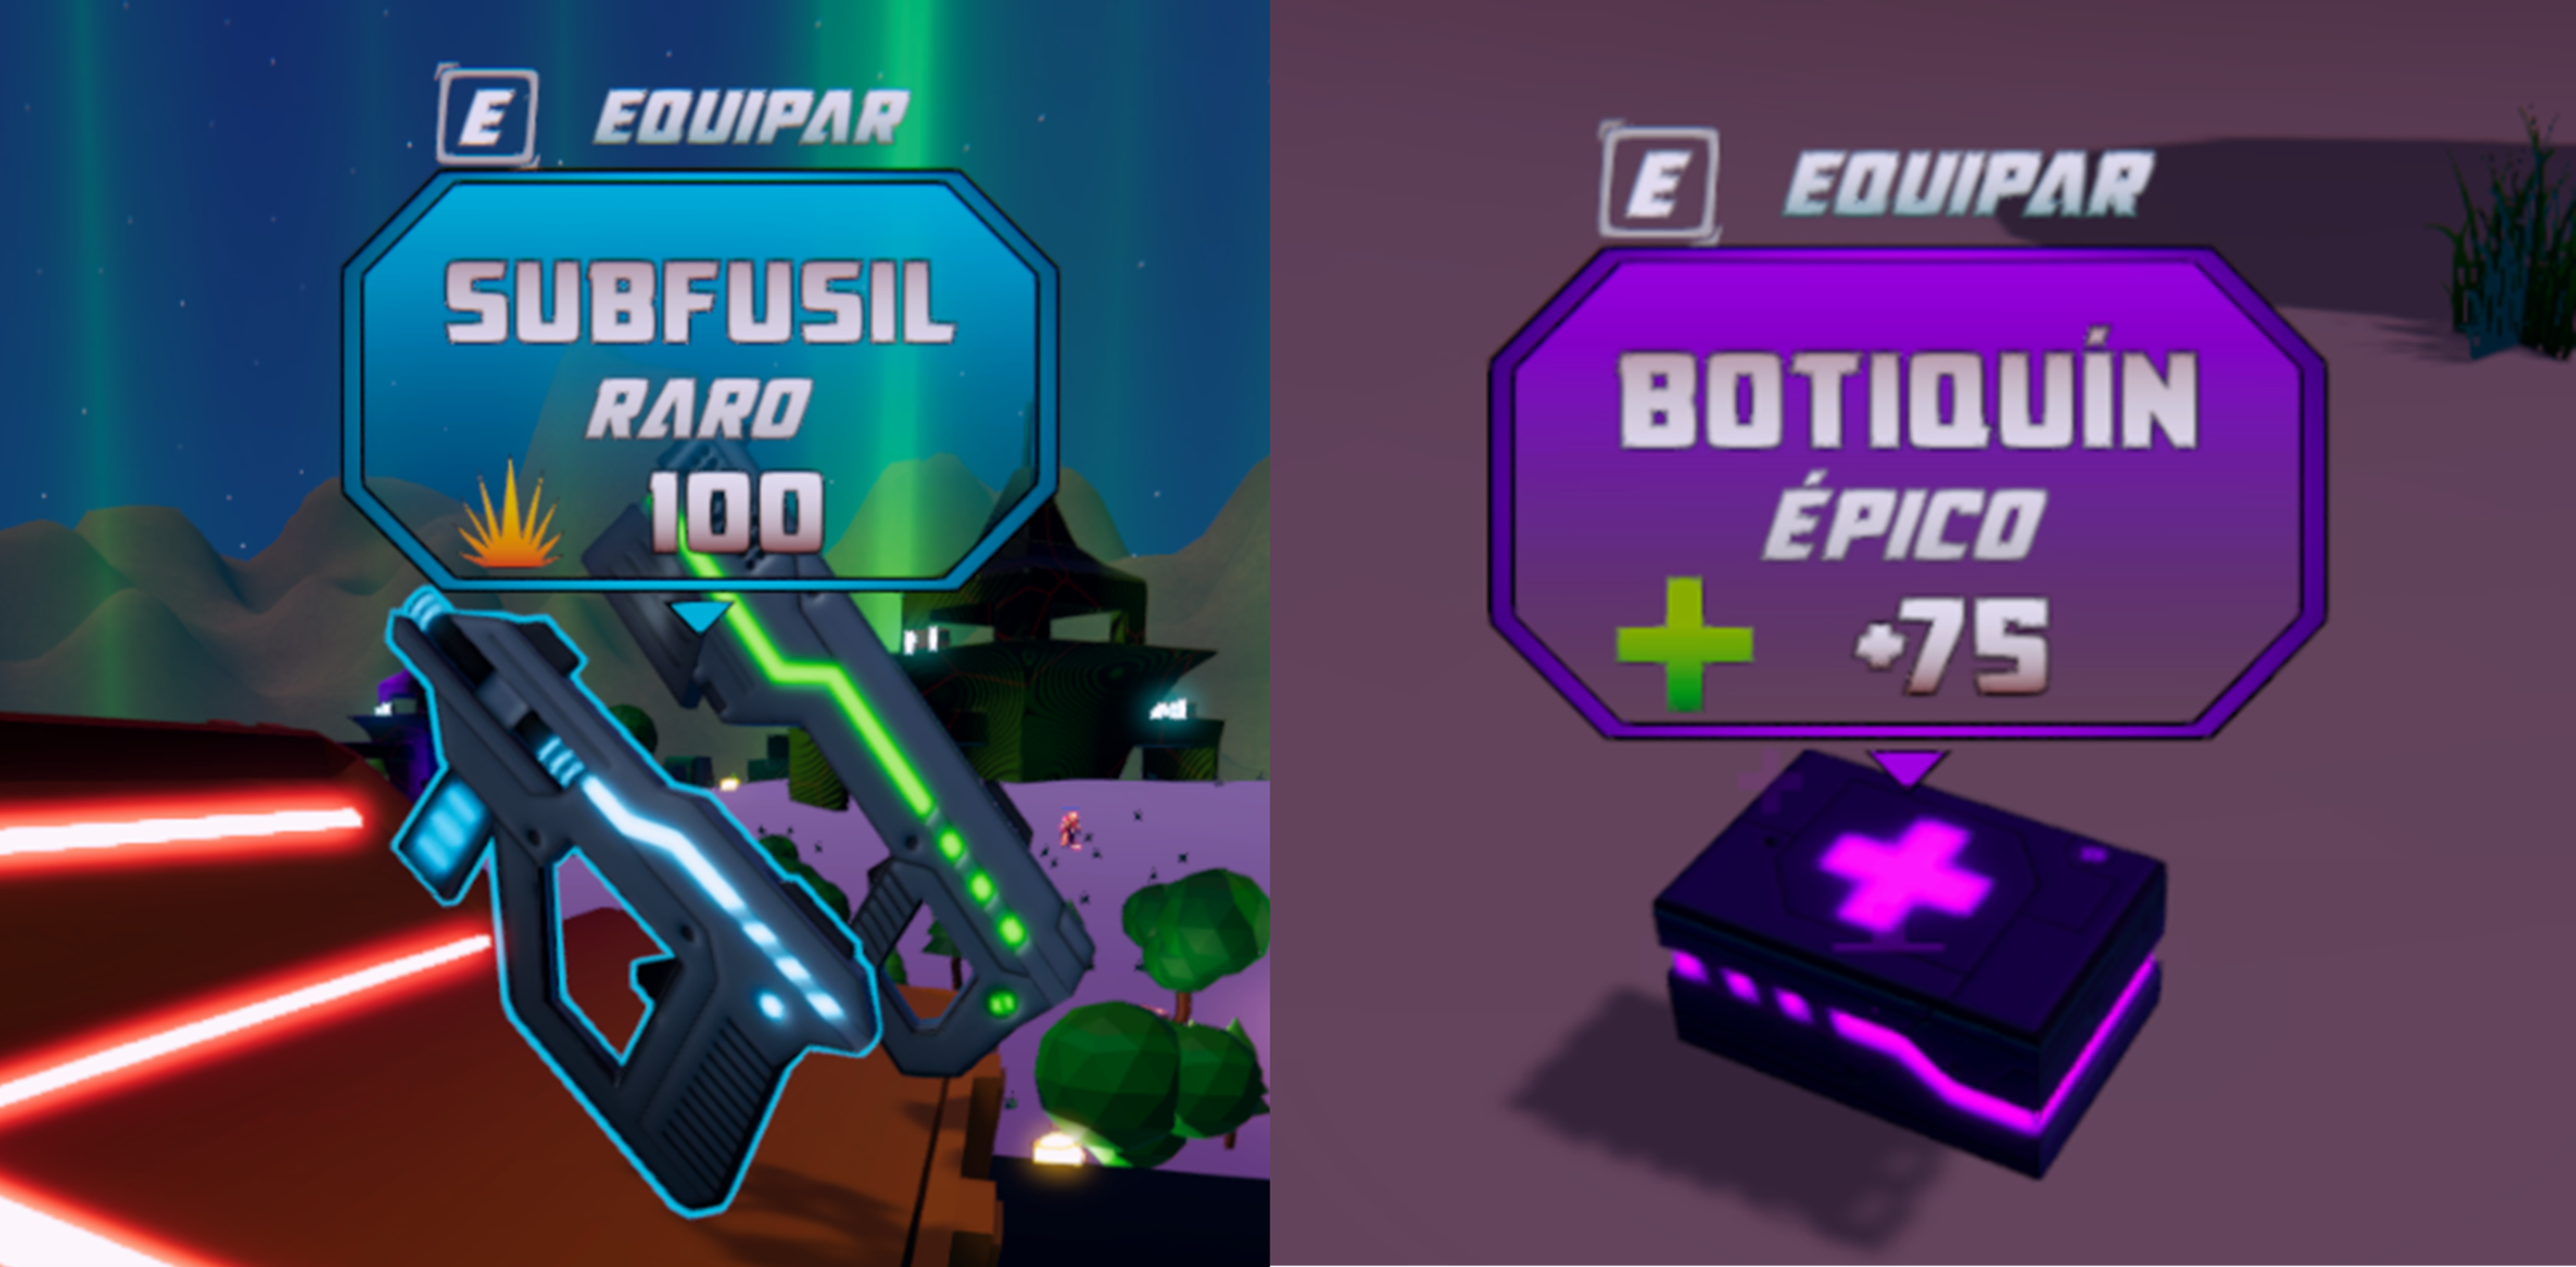
\includegraphics[scale=0.45]{img/LabelExamples.png}
	\caption{mismo prefab de etiqueta con diferentes valores en función del objeto}
	\label{fig:EjemplosEtiqueta}
    \end{figure}
De esta forma, se consigue tener un objeto ``plantilla'' a partir del cual poder crear cualquier etiqueta que se desee simplemente dando valores a los campos, lo que responde, ahora sí, al principio de eficiencia y extensibilidad del proyecto.

\section{Apartado visual y postprocesado}
Para conseguir un resultado gráfico más atractivo visualmente, se decidió utilizar \textbf{URP} (\textit{Universal Render Pipeline}), una sistema de renderizado gráfico que introduce mejoras en las características de la línea de renderizado predeterminada de Unity. Integra varias funciones y de iluminación para conseguir un acabado más pulido en el apartado visual del sistema.

Una de las principales ventajas de usar URP es que trae consigo un sistema de postprocesado integrado, a diferencia del sistema de renderizado por defecto, en el que habría que importar paquetes externos para tener opciones similares.
Las funciones de postprocesado funcionan como filtros visuales que se le aplican a las imágenes renderizadas por las cámaras de la escena antes de mostrarlas en la pantalla. Existe una gran variedad de opciones de postprocesado para conseguir distintos efectos en la apariencia final de los fotogramas del juego.

Para añadir estos efectos de postprocesado a una escena con este flujo de trabajo se debe un \textit{\textbf{Volume Profile}} o perfil de volumen de postprocesado. Este es un asset que contiene información sobre los diferentes efectos que se quieran añadir a ese perfil concreto. Por ejemplo, para conseguir la estética futurista que se pretendía tener en este videojuego, es importante que algunas luces tengan un efecto de ``neón''. Algunos objetos que se pretende que tengan este efecto son las cajas de suministros, los enemigos, las partes brillantes de las armas o de las manos del jugador, entre otros.\\
Para lograrlo, se debe añadir el efecto llamado \textit{Bloom}, que hace que las luces se dispersen en los píxeles adyacentes consiguiendo el efecto de brillo deseado. 
URP permite tener no uno sino varios perfiles de postprocesado en la escena para lograr distintos efectos dependiendo de la situación. En el proyecto se han creado cuatro perfiles:
\begin{enumerate}
    \item El primer volumen corresponde a toda la escena, en el que, además del mencionado \textit{Bloom}, se añaden otros efectos como un efecto de viñeta, aberración cromática en los bordes de la pantalla o correcciones de color para conseguir la estética general deseada y mejorar la apariencia de la escena. Este volumen es renderizado por la cámara principal.
    \item El segundo volumen tiene otros ajustes en el efecto de \textit{Bloom}, y se aplica sobre las imágenes renderizadas por la cámara del jugador, es decir, sobre sus manos, las armas y las granadas.
    \item Un tercer volumen se creó para ser aplicado sobre la cámara que renderiza la escena a través de la mira telescópica del francotirador cuando se apunta con él. Los efectos que se han añadido a este perfil son ajustes de color y un efecto de distorsión en la lente. Con ello se pretende simular el efecto real que se produce al observar a través de una mira de ese tipo.
    \item El último volumen se activa cuando el jugador se encuentra en la zona no segura del mapa. Los efectos que tiene son un tinte verde de la imagen, efecto de viñeta y un filtro de ruido visual. Se intenta simular un efecto de nube tóxica, con tonos verdosos y con ruido para intentar avisar al usuario que no debería quedarse allí y que debería volver a la zona segura del mapa.
    \end{enumerate}
\begin{figure}[h]
	\centering
	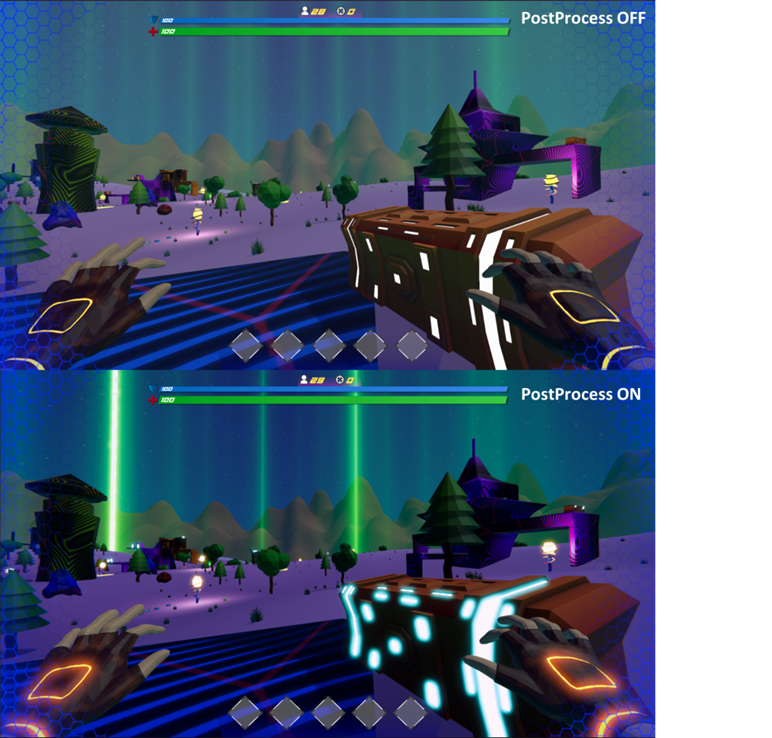
\includegraphics[scale=0.45]{img/PostprocessComparison.png}
	\caption{Deferencia visual de utilizar efectos de postprocesado en la imagen}
	\label{fig:Postprocesado}
    \end{figure}
    Gracias al sistema de renderizado URP y a los perfiles de postprocesado, se consigue crear una atmósfera visual agradable y acorde a la estética definida, creando de manera sencilla e intuitiva diferentes entornos y sensaciones para el jugador (ver figura \ref{fig:Postprocesado}).

\section{Disparo de las armas}
Un dilema al que se enfrentó el alumno al comenzar el proyecto fue el modo en que se dispararían las armas para hacer daño a los enemigos.

En los videojuegos de género \textit{shooter}, suele haber dos técnicas para ello. La primera y más intuitiva consiste en que, al momento de disparar, se instancie un pequeño proyectil a modo de bala que saldrá impulsado hacia delante, asemejándose a como funciona un arma en la realidad. Después se detectaría si el proyectil impacta en un enemigo para infligir el daño correspondiente.

La segunda técnica, usada en el proyecto, se denomina ``Raycasting'' \cite{wiki:Raycast}. Lo que hace Unity con esta técnica es lanzar un rayo desde y hacia donde se desee, y detectar si el rayo colisiona con un enemigo, para que reciba el daño acorde al arma seleccionada.

Se eligió esta última técnica por varias razones:
\begin{itemize}
    \item Se tiene una mayor \textbf{precisión} al disparar, ya que el rayo colisiona con su objetivo prácticamente al instante de disparar, haciendo que el jugador tenga más sensación de control sobre las armas.
    \item Tiene un mejor  \textbf{rendimiento}, al no tener que instanciar un objeto cada vez que se apriete el gatillo, algo que en un shooter como este ocurrirá con mucha frecuencia.
    \item Es un método que, si bien al principio es más complicado de entender, al final resulta más  \textbf{sencillo de mantener}. Es menos propenso a errores, ya que al ser un rayo ``invisible'', se evitan problemas de colisiones, y, en general, de cualquier aspecto a nivel de físicas.
\end{itemize}

Una ventaja de esta técnica es que las armas que sostiene el jugador son solo un elemento visual del juego, y no son realmente funcionales en términos de disparo. El rayo del raycast,  es decir, el disparo real, proviene del centro de la cámara del jugador, y se dirige hacia delante en busca de un collider objetivo. De esta manera se consigue separar la parte lógica de la parte visual, consiguiendo una modularidad estructural que siempre es beneficiosa en este tipo de proyectos para evitar errores o detectarlos y corregirlos más rápidamente.

Una desventaja del raycast es que, al ser invisible, no hay feedback visual de que la ``bala'' ha sido disparada. Sin embargo, este problema se ha solventado añadiendo diferentes efectos y partículas. Por ejemplo, cada arma, al disparar, tiene un retroceso dependiendo de la clase que sea. También se añaden efectos visuales como un fogonazo en la punta del cañón del arma, así como un efecto de impacto cuando el raycast encuentre un collider a su paso. Finalmente, el arma emite un sonido para completar la sensación de disparo real.

\section{Camera clipping}
Un problema habitual al que se enfrentan los videojuegos en primera persona como este, en los que el personaje sujeta algún objeto en su mano, es el llamado \textit{camera clipping}. Este es un efecto visual que ocurre cuando el jugador se acerca demasiado a una pared u obstáculo, haciendo que el parte del objeto que esté sujetando, atraviese la pared, perdiendo así la sensación de realismo del juego. Para no sacar al jugador de la experiencia, hay que conseguir que los objetos que sostenga el personaje, como las armas, se mantengan siempre visibles para el jugador, sin importar cuán cerca esté una pared de él.

La técnica utilizada para resolver este problema consiste en tener dos cámaras separadas. Una se encargará de renderizar toda la escena excepto los objetos que se encuentren en la capa (\textit{layer}) ``Weapon''. La segunda cámara, por contra, solamente renderiza dichos objetos de la capa ``Weapon''. En esta capa se incluyen todos los objetos que el jugador puede sostener en sus manos, como armas, granadas o las propias manos del jugador. De esta manera, primero se ``pinta'' en la pantalla el escenario, los edificios, las paredes y demás elementos generales, y después, por encima, se muestra el objeto sujetado por el jugador. 

De esta manera, no importa cuánto se acerque el jugador a una pared, sus manos y el objeto que sostenga siempre se verán delante de ella (ver figura \ref{fig:ComparacionCamaras}).

\begin{figure}[h]
	\centering
	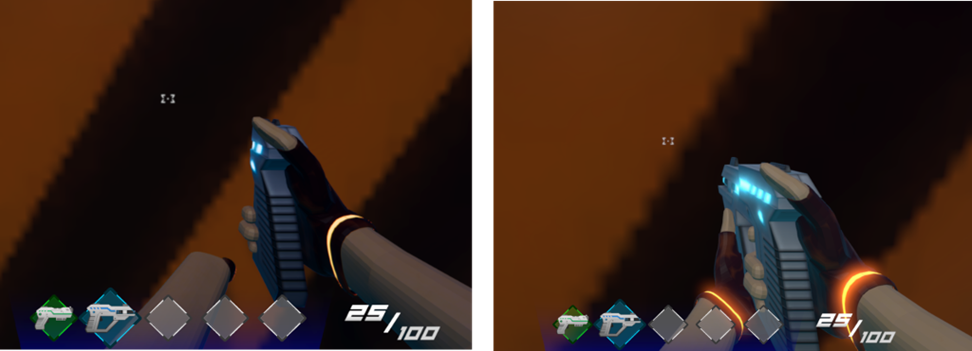
\includegraphics[scale=0.45]{img/CameraClippingComparison.png}
	\caption{Comparación entre usar solo una cámara (izquierda) y usar dos (derecha)}
	\label{fig:ComparacionCamaras}
    \end{figure}
    
\section{Técnicas de optimización}
Además de la optimización inherente al buen diseño de código junto con el uso de patrones de diseño, en el proyecto se han utilizado técnicas específicas de optimización para mejorar el rendimiento general de la aplicación.
\subsection{Normal maps}
En ocasiones se necesita que los modelos de los objetos tengan pequeños elementos o ciertos detalles en su geometría, como arañazos, bultos, surcos, arrugas o incluso relieves más complejos como tornillos, por ejemplo.

El problema es que hacer estos detalles en los modelos con geometría real puede generar demasiados polígonos, incluso en elementos muy pequeños que no se van a apreciar cuando el jugador esté en la partida.
Para solventar este exceso de polígonos que podrían lastrar el rendimiento de la aplicación de manera innecesaria, se utilizan los mapas de normales.
Los mapas de normales o \textit{normal maps}\cite{wiki:NormalMaps} son un tipo de textura especial que permite agragar detalles a las superficies de los objetos de manera artificial, jugando con las normales del objeto y con la luz para representar estos detalles como si estuviesen modelados con geometría real.\\
Para ello, lo que hace es representar con cada pixel de la imagen una desviación en relación a la dirección de la normal de la superficie (una normal es un vector perpendicular al plano tangente a la superficie en un punto). Utilizan los canales de color RGB para representar las coordenadas XYZ, respectivamente, de estas normales de la superficie.

En el videojuego, esta técnica para añadir detalle sin usar más polígonos se utiliza por ejemplo en todas las armas, o en la textura de los enemigos (ver figura \ref{fig:ComparacionNormalMaps})para dar más interés al modelo y que no sea tan plano, sin afectar al rendimiento.

\begin{figure}[h]
	\centering
	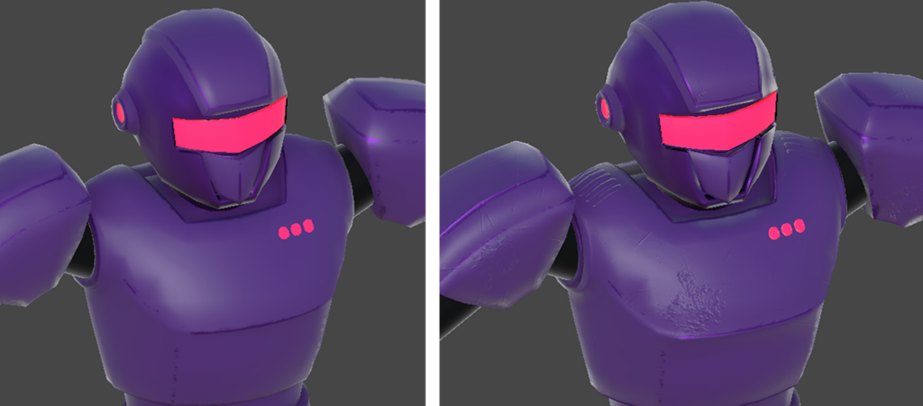
\includegraphics[scale=0.4]{img/NormalMapsComparison.png}
	\caption{Comparación de un modelo sin (izquierda) y con (derecha) \textit{normal maps}}
	\label{fig:ComparacionNormalMaps}
    \end{figure}
    
\subsection{Occlusion Culling}
Este es un proceso de optimización mediante el cual los gamobjects que no sean visibles por la vista de la cámara no se renderizan, es decir, no se cargan en pantalla. Puede que no sean visibles porque se encuentran fuera del rango de visión de la cámara o porque se sitúan detrás de otros gamobjects, manteniéndose ocultos ante la cámara.

Esta técnica mejora en gran medida la fluidez y, en general, el rendimiento de la aplicación, sobre todo en grandes mapas donde hay varios gameobjets conviviendo a la vez.

En el proyecto, durante el inicio del desarrollo, en el que el mapa era estático, se usó esta técnica, y se pensaba utilizar en la versión final. Sin embargo, más adelante se implementó un generador de mapa procedural, que hace que todo el terreno de juego y sus elementos se generen en tiempo de ejecución. 

Como propone la propia documentación de Unity \cite{wiki:OclussionCulling}, esta técnica no es adecuada para este tipo de mapas en los que los elementos se generan de manera dinámica. Para que funcione adecuadamente, deben marcarse desde el editor los gameobjects que puedan ocultar a otros, como estáticos, algo que no se puede hacer una vez iniciada la aplicación.
Por lo tanto, al final se descartó esta técnica de optimización en el proyecto. No obstante, al ser un mapa no muy extenso, con la mayoría de geometrías de estilo \textit{Low-Poly} (Con pocos polígonos), no es una técnica que fuese a marcar una gran diferencia de rendimiento en este proyecto concreto.

\capitulo{6}{Trabajos relacionados}

Existen varios videojuegos de naturaleza similar al proyecto y que han sido tomados como referencia en algunos aspectos durante el desarrollo.

Los videojuegos ``battle royale'' comparten características muy similares en cuanto a mecánicas principales, pero cada videojuego aporta su propia identidad alrededor de ellas, con estilos y funcionalidades distintos en cada caso que hacen que la experiencia de juego sea única.

A continuación se presentan tres videojuegos de este género que han servido de inspiración para este trabajo \cite{wiki:BestBattleRoyale}.

\subsection{Fortnite}
Fortnite es un videojuego creado por la empresa de videojuegos Epic Games que contiene dos modos de juego, uno cooperativo y el modo \textit{battle royale}. Realmente, este juego fue quien dio a conocer este término en la industria de los videojuegos, despertando la curiosidad tanto de otros desarrolladores como de jugadores de conocer en qué consistía este nuevo género. La novedad que supuso en la época, sumado a su estética y a su modelo de negocio ``Free to play'', llevó a Fortnite al éxito, hasta tal punto de convertirse en uno de los videojuegos más populares alrededor del mundo.

Si bien este no es un juego con una perspectiva en primera persona, sí comparte otras similitudes con el trabajo desarrollado: Tiene una estética estilizada, caricaturesca y colorida, que llama mucho la atención, especialmente en el público más joven, algo que en parte se ha tomado como referencia para definir la estética del proyecto. Algunos otros elementos que se han tomado como referencia son la estructura visual del inventario, su sistema de rareza de armas o las plataformas de salto que hay en el juego para impulsarse en el aire.

Una mecánica que destaca en este juego y que lo hace diferenciador del resto de juegos del mismo género es que el jugador tiene la capacidad de construir todo tipo de estructuras. Paredes, rampas o suelos son algunas cosas que puede colocar alrededor de él para refugiarse, cubrirse de los enemigos o llegar a lugares elevados fácilmente.

Además, como es propio de este género, en cada partida participan 100 jugadores, y tiene un elemento, la ``tormenta'', que hace daño a los jugadores, delimitando la zona segura del mapa que se va reduciendo y cambiando de lugar durante la partida.

\subsection{PUBG}
PUBG: Battlegrounds es un juego de la compañía PUBG Studios que también pertenece al género \textit{battle royale}. En este caso, pretende conseguir una experiencia más realista, con armas y equipamiento que existen en la vida real, con complementos intercambiables como miras, cargadores, modos de disparo o silenciadores.

Su diseño y estética también están enfocados en una línea realista, tratando de imitar a la realidad con los efectos visuales y de sonido, gráficos detallados, y un mapa muy amplio con elementos verosímiles. Este juego está más orientado para los jugadores que buscan una experiencia de juego más pura y fiel a la realidad.

Al ser un \textit{battle royale}, en cada partida participan 100 jugadores y el mapa va reduciendo su área segura con el tiempo hasta que solo quede un jugador.
Cabe destacar que el modo de juego puede alternarse entre primera y tercera persona según la preferencia del jugador.

\subsection{Apex Legends}
Apex Legends es un videojuego también \textit{battle royale}, desarrollado por Electronic Arts que de alguna manera combina elementos de los juegos descritos anteriormente. Tiene un tono ciertamente desenfadado, con una estética futurista y algo estilizada, junto con elementos más realistas como el estilo de las armas o un sentido de la estrategia algo mayor que en Fortnite por ejemplo.

Un elemento característico de este popular juego es que los jugadores deben elegir una ``leyenda'' al iniciar una partida. Las leyendas son distintos tipos de personajes, cada uno con habilidades y ventajas propias que le ayudarán durante la partida.

Al igual que en el resto de títulos del género, los jugadores deben situarse en una zona determinada del mapa para no recibir daño. Tiene mecánicas de movilidad interesantes como el poder deslizarse por largas colinas o agarrar tirolinas y lanzaderas para desplazarse más rápidamente por el mapa.

Dos elementos que han servido de inspiración para el trabajo son las cajas de suministros que hay repartidas por el mapa con objetos de interés para el jugador, y el \textit{HUD} flotante que aparece junto a un enemigo cuando se le inflige daño con el color y el número apropiados.

\capitulo{7}{Conclusiones y Líneas de trabajo futuras}

A modo de cierre, se van a exponer las conclusiones finales que se han extraído sobre la realización de este proyecto, así como las líneas de trabajo propuestas por el alumno a realizar en un futuro para continuar y mejorar el desarrollo del mismo.

\section{Conclusiones}
Una vez finalizado el desarrollo de este proyecto, se han extraído algunas conclusiones dignas de mencionar.

En cuanto a los requisitos y objetivos que se marcaron para este proyecto, se han cumplido todos ellos de manera satisfactoria, incluso a un mayor nivel de lo esperado en un principio.
Se ha conseguido, siendo una sola persona, realizar un videojuego completo, con múltiples mecánicas, una buena jugabilidad, sistemas procedurales que hacen que cada partida sea única, con menús e interfaces diseñadas de cero, opciones de personalización, conexión a una base de datos y un sistema de autenticación de usuarios.

Gracias a la combinación de mecánicas, animaciones, sonidos, efectos visuales y movimientos de cámara, se ha logrado cumplir satisfactoriamente todos los objetivos.
Al fin y al cabo, el objetivo principal de un producto software como este es que resulte divertido de jugar, y que la experiencia de uso sea agradable e inmersiva, haciendo que el jugador sienta que todos los elementos funcionan como espera.

Se ha conseguido obtener un videojuego muy disfrutable para toda clase de público al que le guste los retos y la acción, que pone a prueba la puntería, así como la capacidad de estrategia y exploración del jugador.

Además, gracias al desarrollo de este proyecto, se ha obtenido otra perspectiva desde la que observar los videojuegos, fuera del rol de jugador. Se ha comprendido la gran magnitud que tienen este tipo de productos a nivel profesional, y que el hecho de que su desarrollo se lleve a cabo por grandes equipos multidisciplinares es algo inevitable para poder entregar un software de calidad en los escuetos plazos que suelen marcarse en esta industria.

Este proyecto ha sido una forma ideal de aplicar y aunar varios de los conocimientos adquiridos durante la carrera, al tiempo que se crea un producto concreto y funcional de gran interés para el alumno.

\textbf{\textit{The Only One}} es un proyecto que requería una implicación muy grande por parte del alumno, aún más si se tiene en cuenta la escasa experiencia del tutor con proyectos de este tipo, enfocados al desarrollo de un videojuego. El alumno, de manera autónoma, ha investigado y encontrado soluciones ante numerosas cuestiones y situaciones que ponían en aprietos al proyecto. Ha conseguido implementar y adaptar mecánicas, interfaces, modelos, animaciones, sonidos, efectos visuales y otros elementos para hacer que el desarrollo avanzara adecuadamente, acorde a los objetivos fijados.

Se ha conseguido asentar unas bases firmes en materia del desarrollo de videojuegos con las que se espera construir productos de cada vez más calidad de aquí en adelante.

\section{Líneas de trabajo futuras}

Debido a la limitación temporal de este proyecto, se da por finalizado su desarrollo por el momento, consiguiendo haber creado un producto software completamente funcional.
Sin embargo, existen algunas líneas de trabajo futuras que sería interesante desarrollar de aquí en adelante y que aportarían un gran valor al videojuego para crear un producto software más completo.\\ Además, dada la complejidad de alguna de ellas, se valora la opción de buscar un grupo de trabajo más amplio que pueda implementar dichas mejoras de forma más eficiente. Las líneas de trabajo consideradas para el futuro son las siguientes:
\begin{itemize}
    \item La funcionalidad que se tiene como prioridad para desarrollar en el futuro es implementar un \textbf{modo multijugador}. En el género \textit{battle royale}, es habitual poder competir contra otros jugadores reales, incluso con amigos, y así tener una sensación más realista al jugar una partida. Los enemigos actuales tienen una “inteligencia” limitada, lejos de la de una persona real. Cuando se compite contra otras personas, surgen enfrentamientos más interesantes, con estrategias de juego más elaboradas y distintos niveles de juego en función de la experiencia con el juego.
    \item Mejorar la \textbf{inteligencia de los enemigos}. En caso de no implementarse el modo multijugador, sería conveniente añadir mejoras en el comportamiento automático de los enemigos. Es cierto que el sistema actual funciona bien, y crea la sensación de que realmente los enemigos interactúan con el resto de entidades como lo haría un jugador real. Sin embargo, una vez se descubre su funcionamiento interno, es relativamente sencillo adecuarse a su comportamiento para salir victorioso de los enfrentamientos.\\
    Lo ideal es que, en lugar de un sistema tan cerrado y definido como el existente, se implemente algún tipo machine learning, como el sistema de aprendizaje por refuerzo de Unity llamado ML-Agents \cite{wiki:MLAgents}. Con él, los enemigos aprenderían con cada partida nuevos movimientos, habilidades y estrategias para, de esta forma, ser menos predecibles y tener una mejor técnica en los enfrentamientos, dando como resultado un nivel de inmersión más profundo y real.
    \item Incluir nuevos tipos de \textbf{armas}, como lanzacohetes, ametralladoras o incluso armas cuerpo a cuerpo, como cuchillos o espadas, para crear nuevos tipos de enfrentamientos, más variados e interesantes.
    \item Incluir nuevos tipos de \textbf{granadas} para aportar una jugabilidad más variada.
    
    Algunos conceptos de granadas que se tienen en mente son los siguientes:
    \begin{itemize}
    \item Granadas eléctricas que aturdan e inmovilicen a los enemigos durante unos segundos.
    \item Granadas de veneno, que dejen un charco tóxico que haga daño a quien se encuentre sobre él.
    \item Granadas de impulso que permitan a los jugadores impulsarse una gran distancia como si se subieran a una plataforma de salto.
    \end{itemize}
    \item Implementar un sistema de potenciadores o \textbf{\textit{power ups}}, objetos especiales que el jugador puede equipar o consumir, otorgándole diversas ventajas sobre el resto por unos segundos, como poder correr más rápido, saltar más alto, hacerse invisible o ralentizar el tiempo. Crearía nuevas dinámicas y estrategias que aportarían más diversión al juego,
    \item Pulir \textbf{aspectos visuales}, como los modelos, la iluminación, las texturas, así como el \textit{HUD} o  las interfaces de los menús, para mantener la armonía estética y la usabilidad, ofreciendo una experiencia de usuario limpia y coherente.
    \item Crear un \textbf{sistema de niveles del jugador}, que vaya aumentando según se gane experiencia, desbloqueando aspectos visuales para modificar el aspecto de los brazos, las armas y demás objetos. Estos cosméticos no afectarían a la jugabilidad de la partida, sino únicamente a la apariencia de dichos objetos para adecuarse al estilo del jugador.
    \item Buscar otras formas de hacer que el juego sea viable económicamente para poder \textbf{publicarlo} en alguna plataforma dedicada para ello, como \textit{Steam}. Según la licencia acordada para este proyecto, se debería crear una pantalla especial de créditos para mencionar a los autores de los elementos usados en el proyecto que lo requieren.
\end{itemize}


\bibliographystyle{plain}
\bibliography{bibliografia}

\end{document}
